\documentclass[a4paper, 11pt]{article}

% Packages
\usepackage{graphicx}
\usepackage[margin=1in]{geometry}
\usepackage[utf8]{inputenc}
\usepackage[T1]{fontenc}
\usepackage[backend=bibtex]{biblatex}
\usepackage{comment}
\usepackage{hyperref}
\usepackage{amsmath}

\usepackage{CJKutf8}

\addbibresource{references.bib}

\title{Evaluation of Machine Translation Pre-Trained Models for Many-to-English Translation}
\author{Stefan Liemawan Adji}
\date{\today}

\begin{document}


\maketitle


\begin{abstract}
    Machine translation (MT) has become an essential tool for overcoming language barriers in an increasingly globalised world. Today, there are pre-trained models specifically designed for automatic machine translation. This paper evaluates the performance of various machine translation pre-trained models (MT-PTMs) for many-to-English translation. The models assessed include OPUS-MT \cite{tiedemann-2020-opus-mt}, mBART-50 \cite{liu-2020-mbart}, NLLB-200 \cite{nllb200-2020}, and M2M-100 \cite{fan-2020-m2m100}. Using a dataset curated from the Tatoeba repository, comprising 1,323 parallel sentence pairs across 14 source languages, translation quality is measured using BLEU, SacreBLEU, and METEOR scores. The results indicate that OPUS-MT, a one-to-one PTM, outperforms multilingual models in one-to-English translation tasks, with mBART-50 leading among the multilingual models. Chinese, Italian, Polish, and Turkish translations to English show the best performance on average across the four models used in this study, however, Ukrainian-to-English on the OPUS-MT model achieves the highest SacreBLEU and METEOR scores.
\end{abstract}

\section{Introduction}

According to Ethnologue \cite{ethnologue-2024}, 7,164 languages currently exist and are in use today, with 40\% of them considered endangered. With so many languages around us, the language barrier has become a known issue, especially in the current globalised world where it is essential for individuals who speak different languages to be able to communicate effectively \cite{nakamura-2009-overcoming}. Thus, the need for translation services to facilitate communication across different languages has also surged \cite{okpor-2014-machine-ta}. As of August 2024, only 243 languages are supported by Google Translate (according to Wikipedia \cite{wikipedia-google-translate}).

Machine translation (MT) refers to the task of automatically translating from one language to another, which typically can be done through text or audio. The research and practice can be traced back to 1949 \cite{weaver-1999}, with the first public demonstration of an MT system on January 7, 1954, in collaboration with IBM, where 49 Russian sentences were translated into English using a limited vocabulary of 250 words and 6 grammar rules \cite{hutchins-2006-first-mt}. However, over the next several decades, growth was limited for machine translation, with 1956-1966 considered the decade of high expectation and disillusion, and 1967-1976 dubbed 'the quiet decade' \cite{hutchins-2001-mt-50-years}. Then in 1989, the dominance of the rule-based approach was challenged by the rise of new methods and strategies, collectively referred to as ‘corpus-based’ methods (data-driven) \cite{hutchins-1994-research-methods-mt,hutchins-1998-development-mt}. Subsequently, statistics-based approaches for MT re-emerged, bolstered by the recent success of probabilistic techniques in speech recognition. Statistical machine translation \cite{lopez-2008-smt} dominated the domain between the late 1990s through the early 2010s, before largely being surpassed by neural machine translation (NMT) \cite{cho-2014-properties,sutskever-2014-seq2seq}.

Since the introduction of Transformers in 2017 \cite{vaswani-2017-attention}, Natural Language Processing (NLP) and machine translation in particular reached a giant milestone. The following years saw the birth of Large Language Models (LLMs) such as BERT \cite{devlin-2019-bert}, GPT \cite{openai-2024-gpt4}, and T5 \cite{raffel-2023-t5}, which revolutionised both MT and the whole field of NLP. Then in the early 2020s, several pre-trained models that are specifically designed for machine translation emerged, these will be referred in this paper as Machine Translation Pre-Trained Models (MT-PTMs). OPUS-MT \cite{tiedemann-2020-opus-mt} produced numerous models designed for one-to-one translations. Additionally, multilingual models: mBART-50 \cite{liu-2020-mbart}, NLLB-200 \cite{nllb200-2020}, and M2M-100 \cite{fan-2020-m2m100} have also been published, growing popularity as multilingualism has been shown to allow for sharing information among languages \cite{garcia-2020-multilingual}. Most of these models are trained on a diverse set of languages, allowing for many-to-many translation, which is able to translate between any of the supported pairs of languages. This allows the models to generalise over shared lexical and linguistic among languages, and have been shown to increase performance compared to one-to-one translation models \cite{liu-2020-mbart}.

Despite these advancements, pre-trained models are often evaluated using a different set of languages and benchmarks \cite{liu-2020-mbart,nllb200-2020,fan-2020-m2m100,wei-2023-polylm}, making it difficult to gauge their relative effectiveness across various languages. Multilingual datasets often do not contain parallel texts across different language pairs; instead, each language pair typically has its own unique set of texts that may not overlap with the texts available in other languages \cite{tiedemann-2020-tatoeba-challenge,cettolo-2012-wit3}.

Nevertheless, there does not seem to be much work on comparing or benchmarking different MT-PTMs in machine translation. Intento recently published 'The State of Machine Translation 2024' \cite{intento-2024} providing an in-depth evaluation of 52 MT engines and LLMs across 11 language pairs. Figure \ref{fig:intento_quality} shows the reported translation quality across different domains and language pairs, showing that the results significantly varies based on these parameters. They also reported a lack of growth in the number of supported languages and concluded that translation quality significantly varies depending on languages \cite{intento-2024}. However, the biggest drawback in this report is that the selected LLMs are general LLMs such as GPT-4 \cite{openai-2024-gpt4}, LLaMa2 \cite{touvron-2023-llama2}, and Mistral \cite{jiang-2023-mistral-7b}, instead of MT-specific models.

\begin{figure}[htbp]
    \centering
    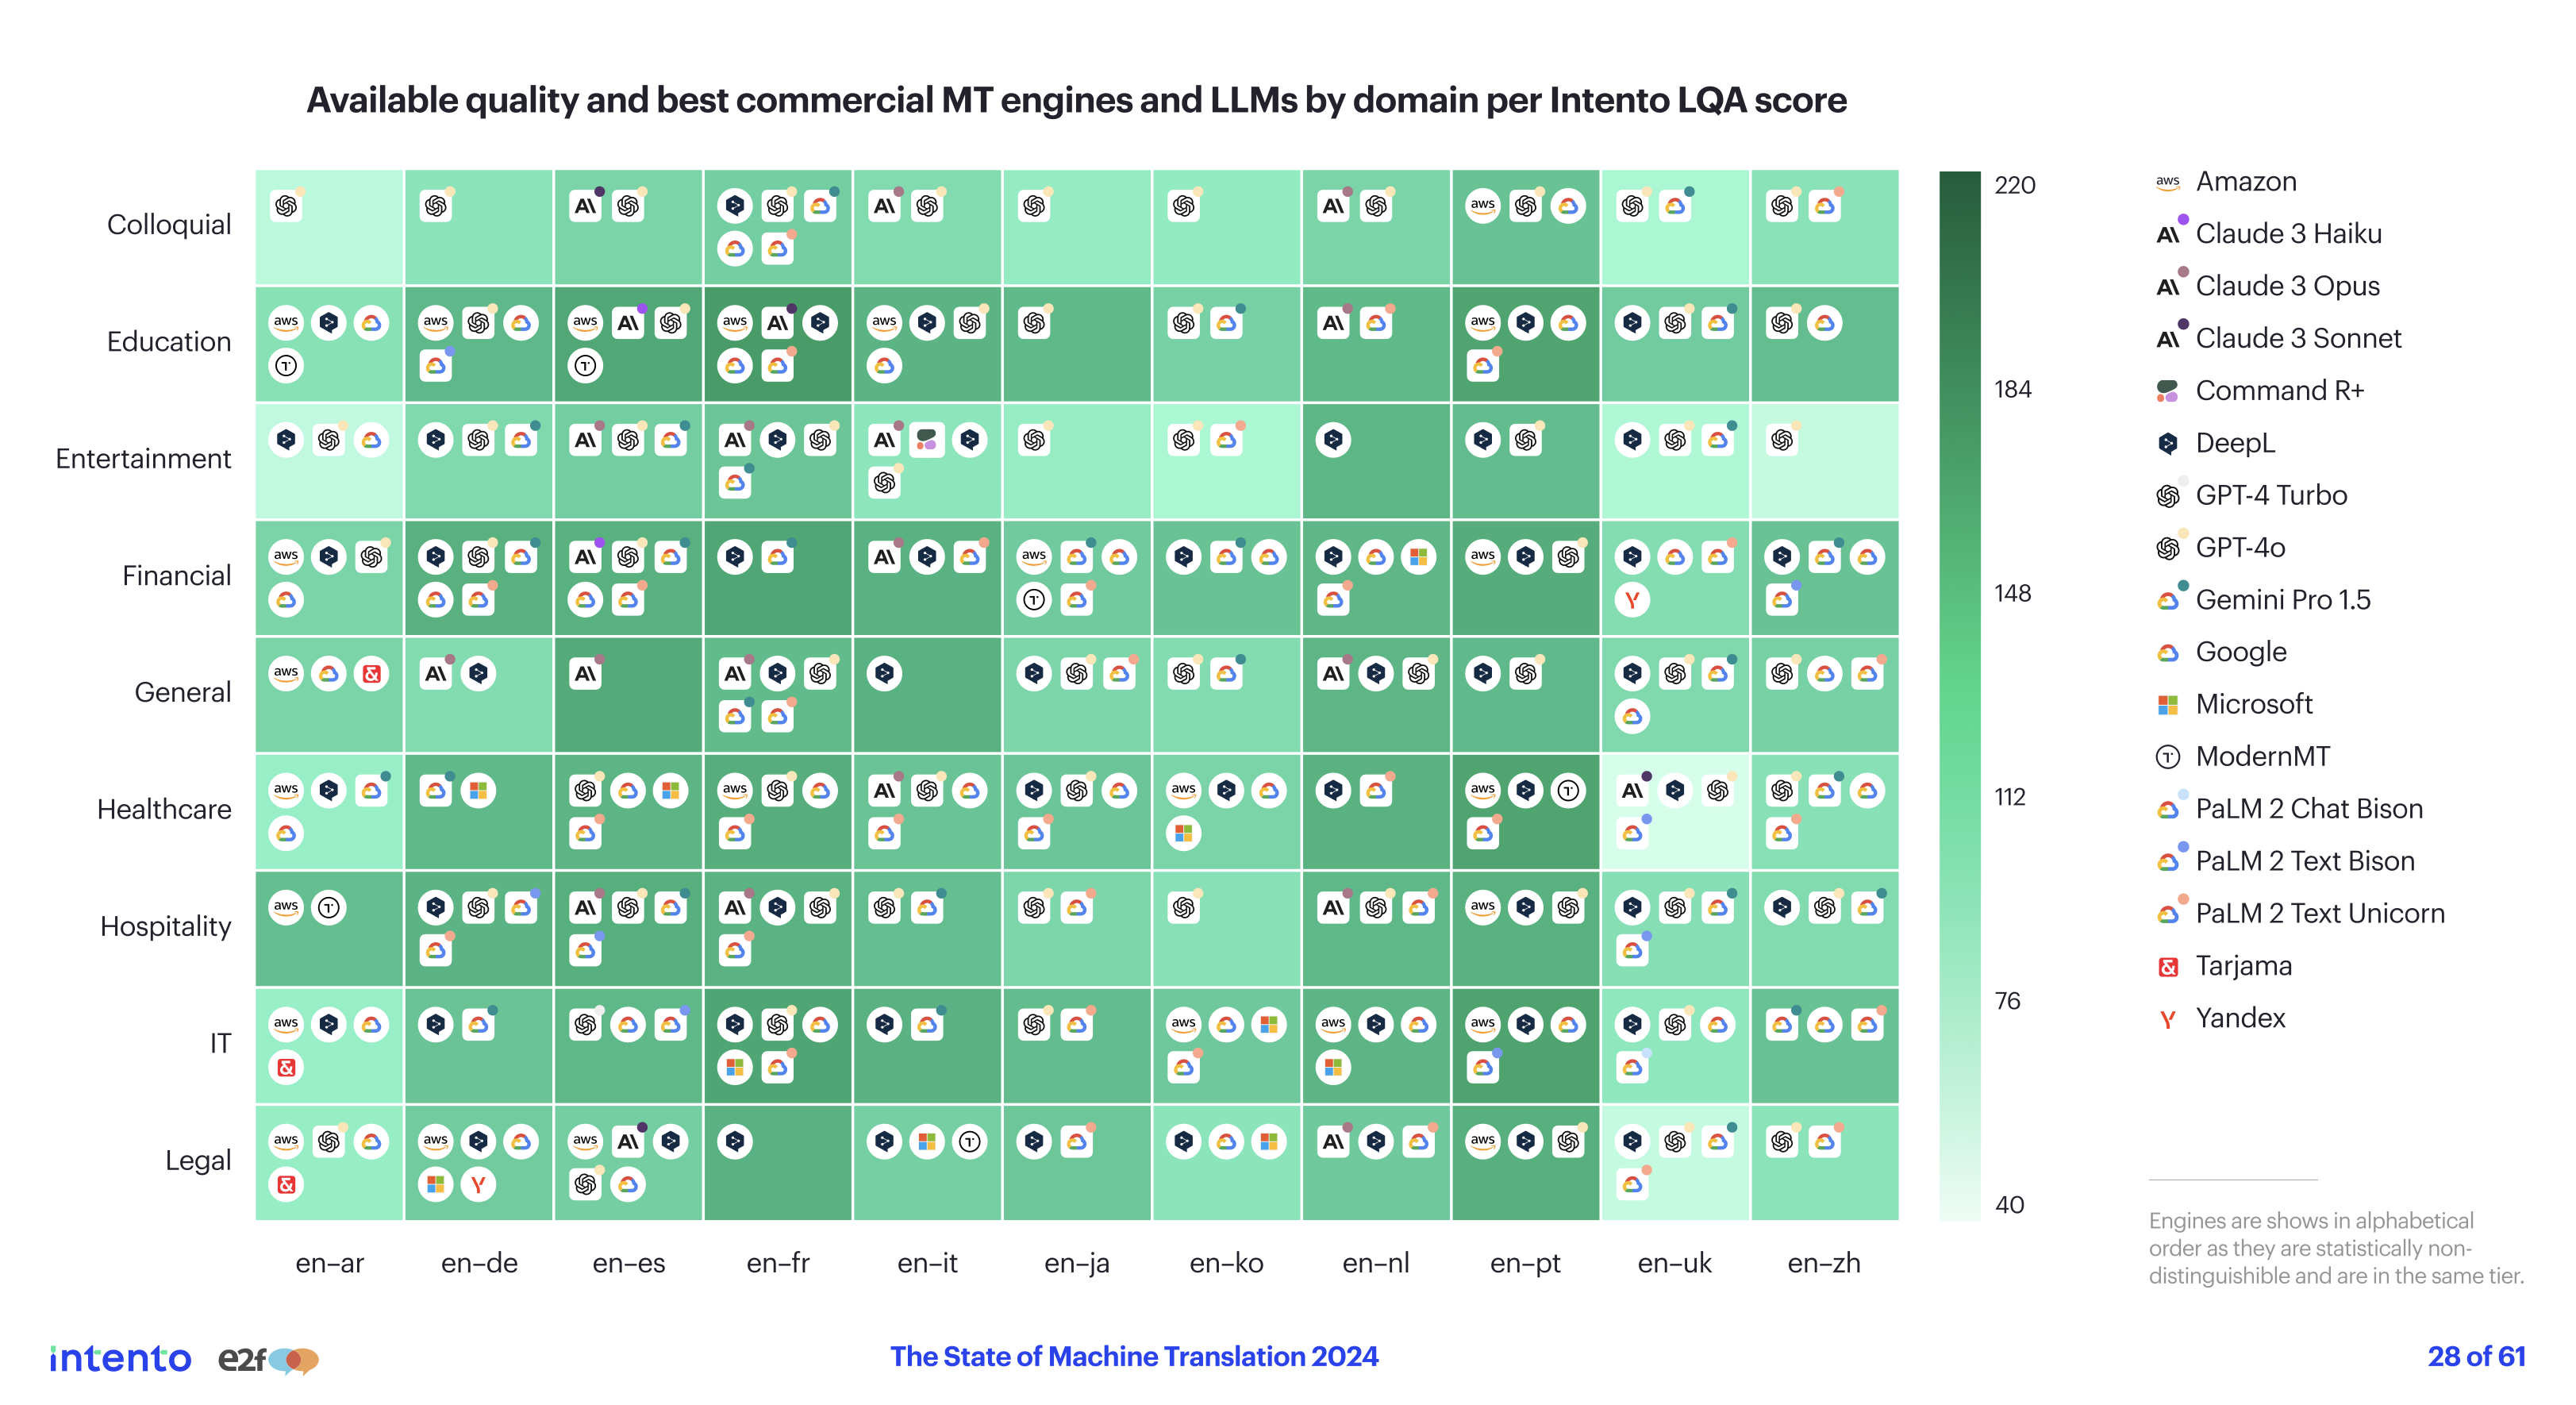
\includegraphics[width=1\linewidth]{images/intento_quality.png}
    \caption{Quality of MT engines and LLMs by domains (y-axis) and language pairs \cite{intento-2024}}
    \label{fig:intento_quality}
\end{figure}

Furthermore, BLEU \cite{papieni-2002-bleu} has been shown to be inconsistent depending on tokenisation and parameters that are used \cite{post-2018-sacrebleu}. While most researchers do report on these specifications explicitly, different BLEU parametrisations between different papers still make a direct comparison challenging to do.

This study will lean towards evaluating MT-specific models rather than general LLMs. Through simple experimentations, this paper aims to evaluate the performance of existing and publicly available MT pre-trained models (MT-PTMs) on many-to-English translation across 14 source languages. Although fine-tuning multilingual MT-PTMs has been proven to increase translation performance \cite{cooper-stickland-2021-recipes}, no pre-training or fine-tuning is performed in this study due to simplicity reasons and resource limitations. A dataset is curated from the Tatoeba repository \cite{tatoeba}, containing 1,323 parallel sentence pairs across source and target languages. The models include a one-to-one PTMs: OPUS-MT \cite{tiedemann-2023-democratizing,tiedemann-2020-opus-mt}, and multilingual MT-PTMs: such as mBART-50 \cite{liu-2020-mbart}, NLLB-200 \cite{nllb200-2020}, and M2M-100 \cite{fan-2020-m2m100}. The performance of these models is evaluated using the BLEU \cite{papieni-2002-bleu}, SacreBLEU \cite{post-2018-sacrebleu}, and METEOR \cite{lavie-2007-meteor}.

The result indicates that OPUS-MT outperforms all other multilingual models in one-to-English translation on both SacreBLEU and METEOR scores, highlighting the superiority of specific languages MT-PTMs compared to unfine-tuned multilingual MT-PTMs. Among the multilingual models, mBART-50 shows the best performance, while NLLB-200 performs the worst, by a significant margin. Ukrainian-to-English translation by OPUS-MT receives the highest scores, however, Chinese, Italian, Polish, and Turkish are better on average across the four models.

\section{Literature Review}

\subsection{Pre-Trained Models for Machine Translation}

Attention mechanism has been used for Neural Machine Translation (NMT) \cite{bahdanau-2016-nmt-jointly, luong-2015-effective-attention} even before the introduction of the transformer \cite{vaswani-2017-attention}. The Transformer, with its encoder-decoder architecture \cite{vaswani-2017-attention}, has since become the foundational framework for many sequence-to-sequence models in machine translation \cite{cho-2014-properties}. By combining this architecture with training on large datasets, models were able to capture and retain vast amounts of linguistic information, leading to the development of pre-trained models.

Currently, pre-trained models have become a cornerstone in machine translation, achieving state-of-the-art performances \cite{han-2021-ptms}. While general Large Language Models (LLMs) such as BERT \cite{devlin-2019-bert}, GPT \cite{openai-2024-gpt4}, or LLAMA \cite{touvron-2023-llama2} can be used for machine translation tasks, in this study the focus will be towards MT-specific PTMs (MT-PTMs) which are specifically designed, built, and trained for machine translation tasks. Most MT-PTMs typically support two kinds of translations: one-to-one translation and many-to-many translation (multilingual models).

One-to-one translation refers to a translation approach where a model is specifically trained to translate between one source language and one target language. This setup is characterised by having a dedicated model for each unique language pair. OPUS-MT \cite{tiedemann-2020-opus-mt} is a project dedicated to creating and providing free resources for machine translation, providing over a thousand MT-PTMs of direct one-to-one translations. Additionally, Facebook Fairseq \cite{ott-2019-fairseq} similarly offers one-to-one MT-PTMs, although they are only limited to translations between English, French, German, and Russian.

Many-to-many translation allows for a translation between multiple pairs of source and target languages. This is done by training a single multilingual model, typically trained on multilingual datasets. Multilingual models have recently gained significant prominence, shown to be simpler and efficient \cite{aharoni-2019-massively-multilingual}. mBART \cite{liu-2020-mbart}, M2M \cite{fan-2020-m2m100}, NLLB-200 \cite{nllb200-2020}, are examples of massively multilingual models that support many-to-many translation language.

\subsection{Parallel Corpora}

Corpora are large and structured sets of texts used for linguistic research and analysis. Thus, parallel corpora are defined as sets of texts in a given source language along with their translations in another target language \cite{lefer-2020-parallel-corpora}. It can be bilingual or multilingual and is crucial for training and evaluating machine translation. Languages without or with limited parallel corpora are referred to as low-resource languages.

Since the early 2000s, English has often been used as an intermediary language, meaning texts originally written in languages are first translated into English, and then from English into other languages, resulting in most target texts being translations of translations \cite{lefer-2020-parallel-corpora}. This is called indirect translation and poses many problems in translations as terms can be ambiguous with varying or similar meanings \cite{rosa-2017-indirect-translation-problems}.

Neural Machine Translation (NMT) systems require vast amounts of training data, and thus the availability of parallel corpora is crucial for building effective models \cite{koehn-2017-challenges}. The lack of extensive parallel corpora, especially for low-resource languages, leads to suboptimal performance in NMT techniques compared to their high-resource counterparts \cite{ranathunga-2023-nmt-low-res}. OPUS \cite{opus} is a comprehensive collection of open-source parallel corpora used extensively in the field of machine translation (MT). It includes corpora for 744 languages and contains over 1,210 different datasets, amassing a total of 45,945,946,108 sentence pairs. Tatoeba \cite{tatoeba} is another prominent resource in the field of MT and NLP, known for its extensive collection of translated sentences. As of July 2024, it contains 12,186,207 sentences over 423 supported languages, growing daily through volunteer contributions. There are currently
86,915 members contributed through the Tatoeba website.

Several datasets are often used for evaluation in machine translation. The Tatoeba Challenge \cite{tiedemann-2020-tatoeba-challenge} covers 487 languages in 4,024 language pairs, including 657 test sets sourced from the Tatoeba website, covering 138 languages. The TED Talks dataset \cite{ye-2018-word-embeddings-ted} contains transcripts from TED talks for more than 50 languages. IWSLT \cite{agarwal-iwstl-2023} also contains TED talks data, but paired with English translations. Finally, WMT (Conference on Machine Translation) \cite{barrault-2020-wmt}, previously named Workshop on Statistical Machine Translation, is an annual event that organises tasks for machine translation and provides a collection of datasets for benchmarking and evaluating translation systems.

While these datasets can be used to evaluate translation performance between any language pairs, they do not contain parallel corpora between multiple different languages. A corpus between English and French, for example, contains different sets of text than a corpus between English and Spanish. Therefore, they do not support easy evaluation for many-to-English translations. Furthermore, papers often use different datasets and versions to evaluate their model performance, making direct comparisons challenging. mBART \cite{liu-2020-mbart} uses WMT19 for English-German translation and TED15 for Chinese-English translation. M2M-100 \cite{fan-2020-m2m100} uses seven different datasets shared across languages. NLLB-200  \cite{nllb200-2020} uses the FLORES dataset, designed for low-resources languages. OPUS-MT \cite{tiedemann-2023-democratizing,tiedemann-2020-opus-mt} models are evaluated using the datasets from Tatoeba challenges.


\section{Methodology}

\subsection{Dataset}

The Tatoeba website \cite{tatoeba} includes a vast, continuously expanding database consisting of sentences and their translations, built through the contributions of thousands of volunteers. They currently have 12,132,349 sentences of over 423 supported languages, with around one to two thousand new sentences added daily, on average. The English sentence dataset contains 1,905,089 sentences, the largest one in their repository, with Russian in second place with 1,066,633 sentences. Figure \ref{fig:tatoeba_languages} shows the repository, sorted from the biggest corpus.

\begin{figure}[htbp]
    \centering
    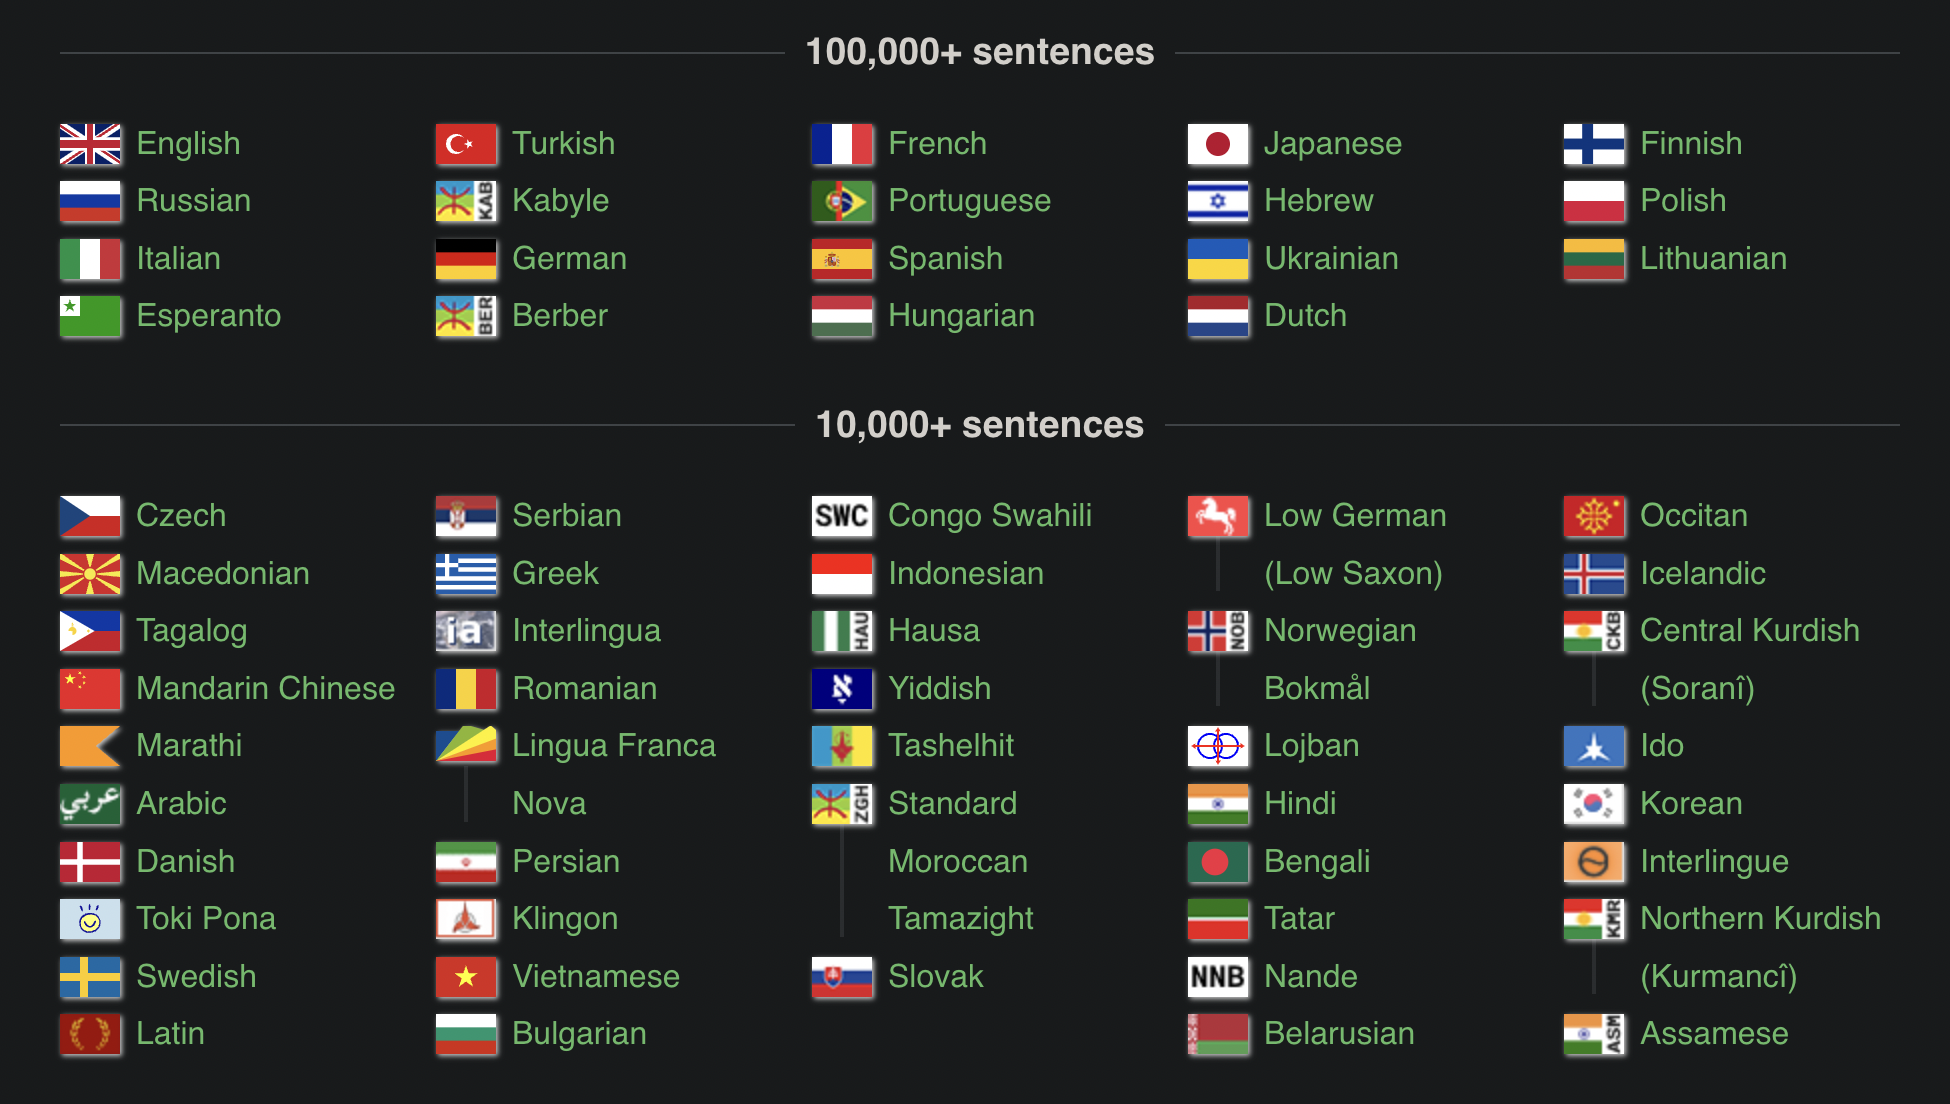
\includegraphics[width=0.65\linewidth]{images/tatoeba_languages.png}
    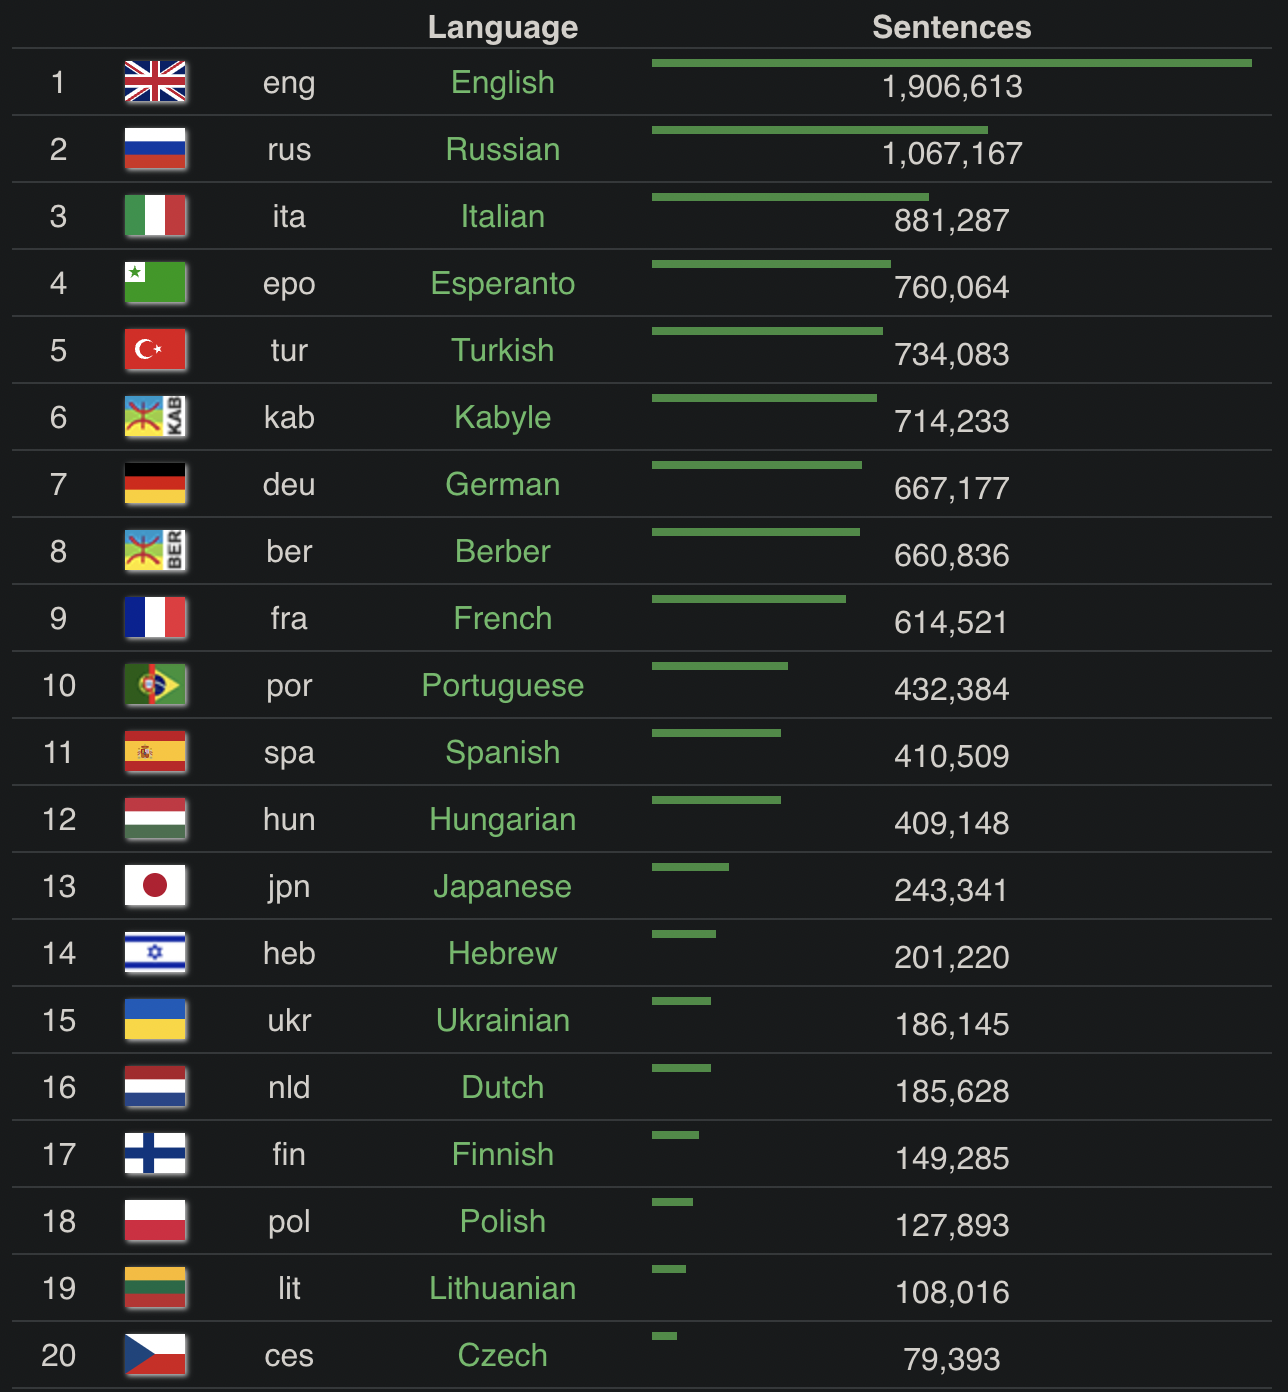
\includegraphics[width=0.34\linewidth]{images/tatoeba_top_20_lang.png}
    \caption{Tatoeba's repository by languages, sorted by sentences count \cite{tatoeba}}
    \label{fig:tatoeba_languages}
\end{figure}

\begin{table}[htbp]
    \centering
    \large
    \begin{tabular}{llr}
        \hline
        \textbf{No.} & \textbf{Language Pairs} & \textbf{Sentence Pairs Count} \\
        \hline
        1            & Chinese-English         & 68,814                        \\
        2            & Dutch-English           & 155,856                       \\
        3            & Finnish-English         & 102,202                       \\
        4            & French-English          & 405,088                       \\
        5            & German-English          & 501,145                       \\
        6            & Hebrew-English          & 172,082                       \\
        7            & Hungarian-English       & 171,698                       \\
        8            & Italian-English         & 624,160                       \\
        9            & Japanese-English        & 270,116                       \\
        10           & Polish-English          & 77,345                        \\
        11           & Russian-English         & 722,837                       \\
        12           & Spanish-English         & 265,253                       \\
        13           & Turkish-English         & 710,279                       \\
        14           & Ukrainian-English       & 214,244                       \\
        \hline
                     & Total                   & 4,461,119                     \\
        \hline
    \end{tabular}
    \caption{List of chosen languages for evaluation}
    \label{table:eval_languages}
\end{table}

Table \ref{table:eval_languages} shows the 14 language pairs selected for this study. Languages are chosen based on the resources' availability in Tatoeba and supported languages in most MT-PTMs. Thus, the languages chosen here can be considered moderate to high-resource languages.

To build the dataset, 1,898,494 English sentences were initially downloaded, though the number is less than what is listed on the Tatoeba website for reasons that remain unclear. For each of the 14 source languages, sentence pairs in English were individually downloaded and compiled. The English corpus was then merged with each compiled source language corpus to create parallel sentences across 14 languages. In each corpus, multiple translations for the same English phrase were dropped, retaining only the first translation to ensure that each English sentence had only a single translation reference. The final dataset contains 1,323 parallel sentences in English and all 14 source languages. This corpus will be used as a test set to evaluate the models' performance in each language.

Sentences typically consist of everyday phrases such as 'I have to go to sleep', 'That is intriguing', and 'Where do you live?'. They may also include single-word exclamations like 'Speak!', 'So what?', or 'Look!'. Additionally, multiple sentences such as 'You may write in any language you want. On Tatoeba, all languages are considered equal', and 'Guns don't kill people. People kill people' can be found inside the corpus. A few of them also include human names, 'Compare your answer with Tom's', and 'Muiriel is 20 now'. All the sentences seem to be straightforward and literal, without any use of linguistic features such as metaphors or sarcasm. Figure \ref{table:parallel_sentence} shows a couple of examples of parallel sentences in the final dataset, across all 14 languages and the original English sentence.

\begin{CJK}{UTF8}{gbsn}
    \begin{table}[htbp]
        \centering
        \begin{tabular}{lrr}
            \hline
            \textbf{Language} & \textbf{Sentence 1}                   & \textbf{Sentence 2}                   \\
            \hline
            English           & I have to go to sleep.                & So what?                              \\
            Chinese           & 我该去睡觉了。                               & 那又怎樣?                                 \\
            Dutch             & Ik moet gaan slapen.                  & Dus?                                  \\
            Finnish           & Minun täytyy mennä nukkumaan.         & Mitä sitten?                          \\
            French            & Je dois aller dormir.                 & Et alors ?                            \\
            German            & Ich muss jetzt schlafen.              & Na und?                               \\
            Hebrew            & <hidden-due-to-latex-incompatibility> & <hidden-due-to-latex-incompatibility> \\
            Hungarian         & Aludni kell mennem.                   & És akkor mi van?                      \\
            Italian           & Devo andare a dormire.                & E allora?                             \\
            Japanese          & 私は眠らなければなりませ                          & だから何?                                 \\
            Polish            & Muszę iść spać.                       & No i co?                              \\
            Russian           & Мне пора идти                         & Так что?                              \\
            Spanish           & Tengo que irme a dormir.              & ¿Entonces qué?                        \\
            Turkish           & Yatmaya gitmek zorundayım.            & Öyleyse ne yapmalı?                   \\
            Ukrainian         & Маю піти спати.                       & Ну то що?                             \\
            \hline
        \end{tabular}
        \caption{A snippet of the dataset}
        \label{table:parallel_sentence}
    \end{table}
\end{CJK}


\begin{figure}[htbp]
    \centering
    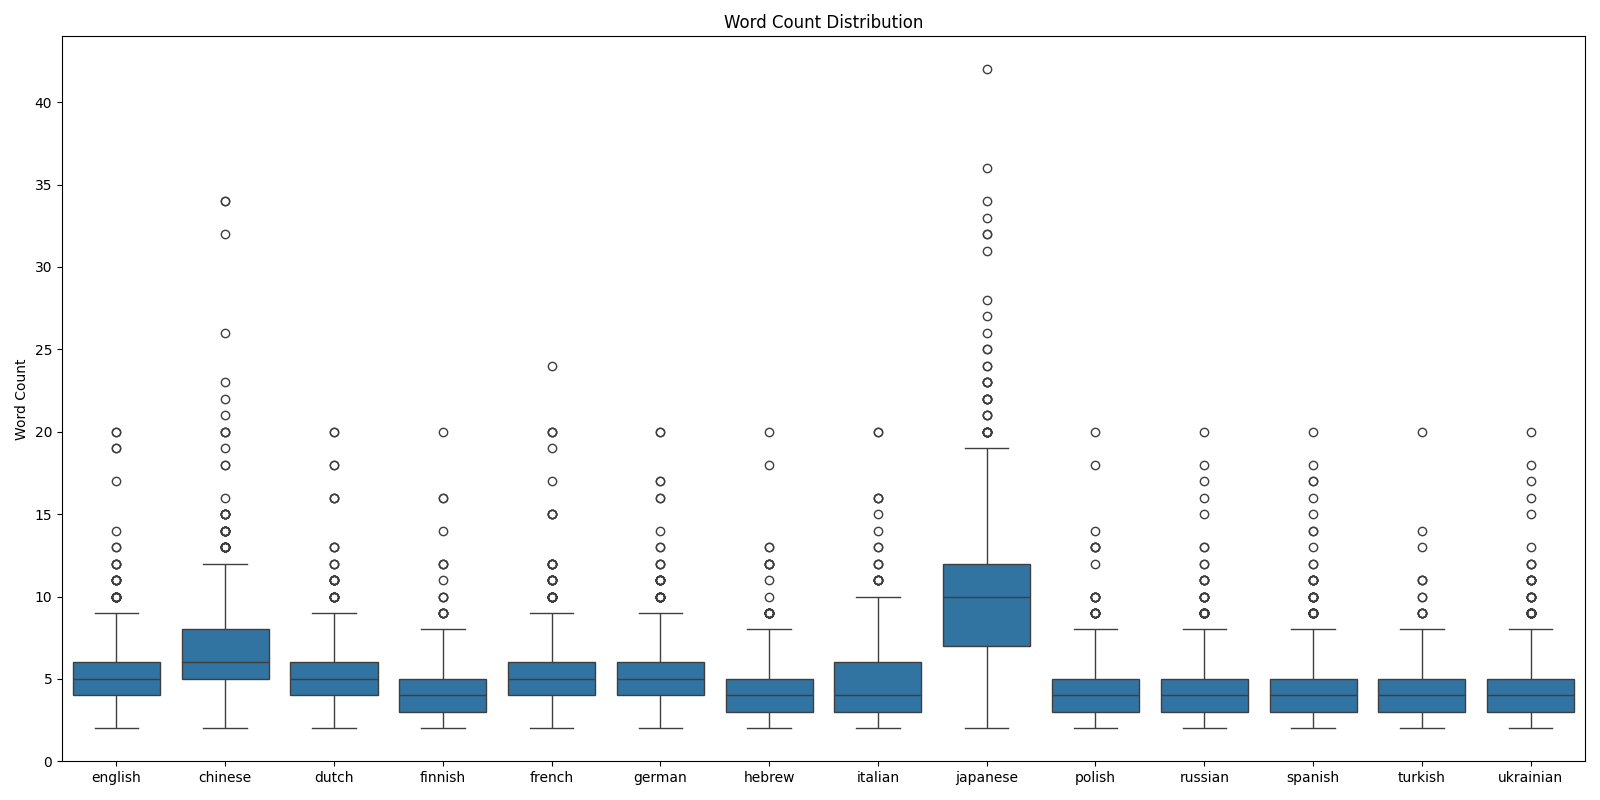
\includegraphics[width=1\linewidth]{figures/word_count_box.png}
    \caption{Dataset word count distribution per language, Chinese and Japanese sentences are counted per letter.}
    \label{fig:word_count_box}
\end{figure}

Figure \ref{fig:word_count_box} shows a box plot of each language sentence's word count. Note that for Chinese and Japanese the word count is counted for each Chinese/Japanese letter instead, which explains their higher range and larger numbers of outliers.

Most of the languages' interquartile range (IQR) is quite low (around two) with a centre median, except for Chinese, Italian, and Japanese. Finnish and Hebrew have the lowest median, while Polish, Russian, Spanish, Turkish, and Ukrainian have a median closely similar to each other. English, Dutch, French, German, and Italian have a slightly higher median, with Italian also having a wider IQR. Lastly, Japanese and Chinese have the highest median, the widest range, and significantly more outliers.

\subsection{Proposed Pre-Trained Models}

\subsubsection{OPUS-MT}

OPUS-MT \cite{tiedemann-2023-democratizing,tiedemann-2020-opus-mt} provides over 1,000 pre-trained models for translation between numerous language pairs. The architecture is based on MARIAN-NMT \cite{mariannmt}, based on a standard transformer setup: 6 self-attentive layers in both the encoder and decoder networks, each with 8 attention heads per layer \cite{tiedemann-2020-opus-mt}. The models were trained for up to 72 hours on 1 or 4 GPUs, noting that not all of them fully converged within this time frame.

While the framework provides both monolingual and multilingual models, only the OPUS-MT monolingual models are used in this study. This is partly due to the lack of documentation on the multilingual models.

\subsubsection{mBART-50}

mBART \cite{liu-2020-mbart} is a sequence-to-sequence denoising auto-encoder model specifically designed for multilingual tasks. The mBART-50 variant supports many-to-many translations for over 50 languages.

\begin{figure}[htbp]
    \centering
    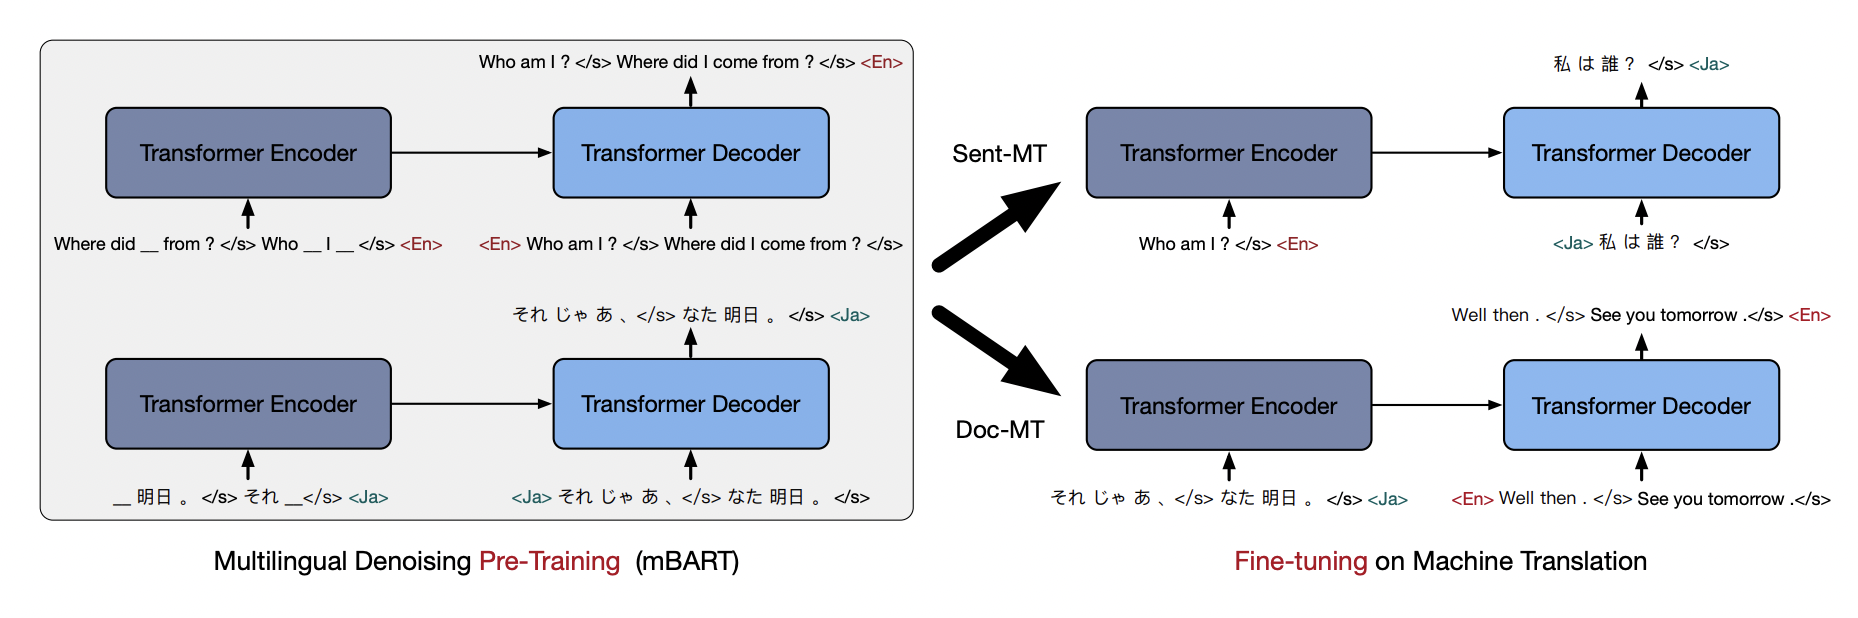
\includegraphics[width=0.9\linewidth]{images/mbart.png}
    \caption{mBART framework for Multilingual Denoising Pre-training (left) and fine-tuning on downstream MT tasks
        (right) \cite{liu-2020-mbart}}
    \label{fig:mbart}
\end{figure}

The mBART model is built as a typical sequence-to-sequence transformer architecture \cite{vaswani-2017-attention}, using an embedding dimension of 1024 and 16 heads within 12 layers of encoder and 12 layers of decoder, totalling around 680M parameters \cite{liu-2020-mbart}.

Figure \ref{fig:mbart} shows mBART's key features: multilingual denoising pre-training and fine-tuning. The dataset is first corrupted by a noising function, which is applied to 35\% of words of each span text \cite{liu-2020-mbart}. During pre-training, the model will be made to denoise the texts, improving the model's ability to generate coherent and accurate translations. After the pre-training step, the model is then able to be fine-tuned for downstream tasks. It is shown that the model achieved consistent performance gains through pre-training in low-to-medium resource sentence-level translation \cite{liu-2020-mbart}

\subsubsection{M2M-100}

M2M-100 \cite{fan-2020-m2m100} is designed to perform direct translation between any pair of 100 languages without relying on English as an intermediate language. Similarly, the architecture is of a transformer sequence-to-sequence with a typical encoder that outputs embeddings of the same length, while the decoder is an autoregressive component that sequentially produces the target sentence one token at a time. The parameters include 12 encoder layers and 12 decoder layers, 8192 hidden layer sizes, and 1024 embedding dimensions, totalling a 1.2B parameter count \cite{fan-2020-m2m100}.

\begin{figure}[htbp]
    \centering
    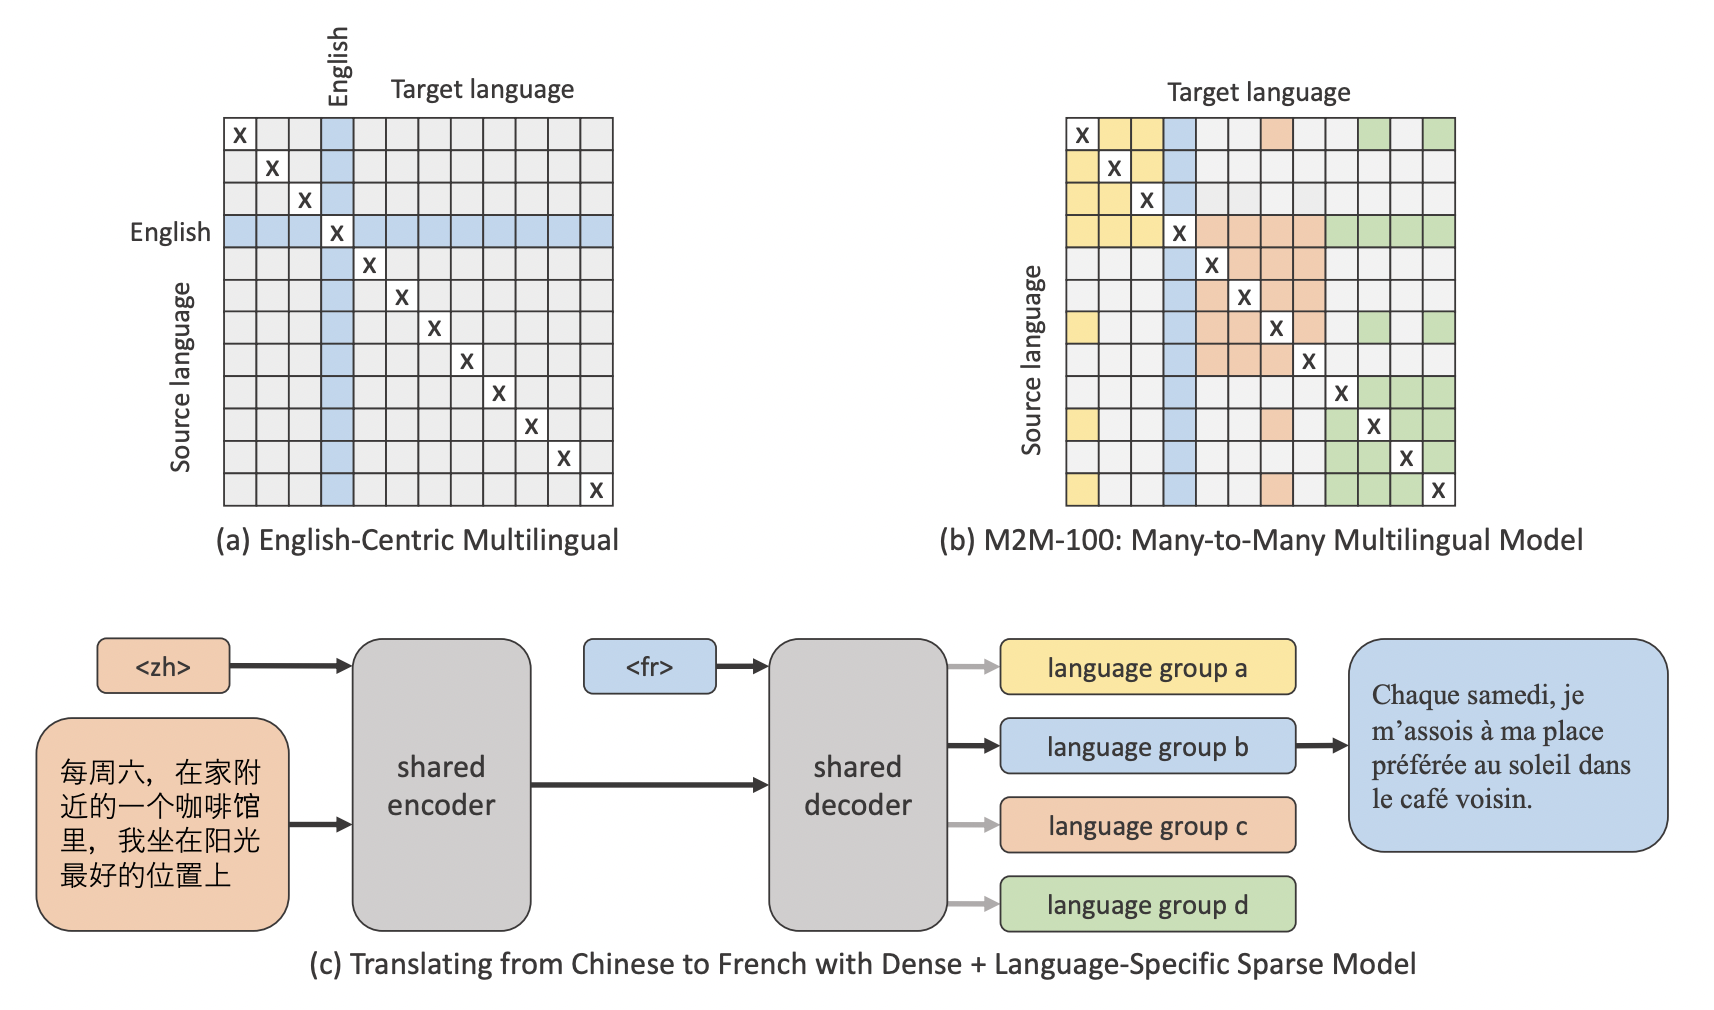
\includegraphics[width=0.9\linewidth]{images/m2m.png}
    \caption{Summary of M2M dataset and multilingual model.}
    \label{fig:m2m}
\end{figure}

Figure \ref{fig:m2m} shows the inner workings of the M2M model. The English-centric dataset (top left) includes training data exclusively involving translations to and from English, while the many-to-many multilingual setting (top right) involves direct translation data among multiple language pairs \cite{fan-2020-m2m100}. Finally, the model combines sparse language-specific parameters with dense parameters (bottom part of Figure \ref{fig:m2m}),

\subsubsection{NLLB-200}

NLLB-200 \cite{nllb200-2020} is built to handle translation tasks across a broad spectrum of languages, including many that are low-resource or underrepresented in existing datasets. It supports translations for 200 languages, including numerous underrepresented languages, and is currently one of the most extensive multilingual machine translation models. The model employs a Mixture of Experts (MoE) architecture and achieves state-of-the-art (SoTA) results across many language pairs, even surpassing Meta's previous model, M2M-100 \cite{nllb200-2020}.

The 'nllb-200-distilled-600M' variant has a total of 600M parameters, distilled from originally 54B parameters \cite{nllb200-2020}

\begin{figure}[htbp]
    \centering
    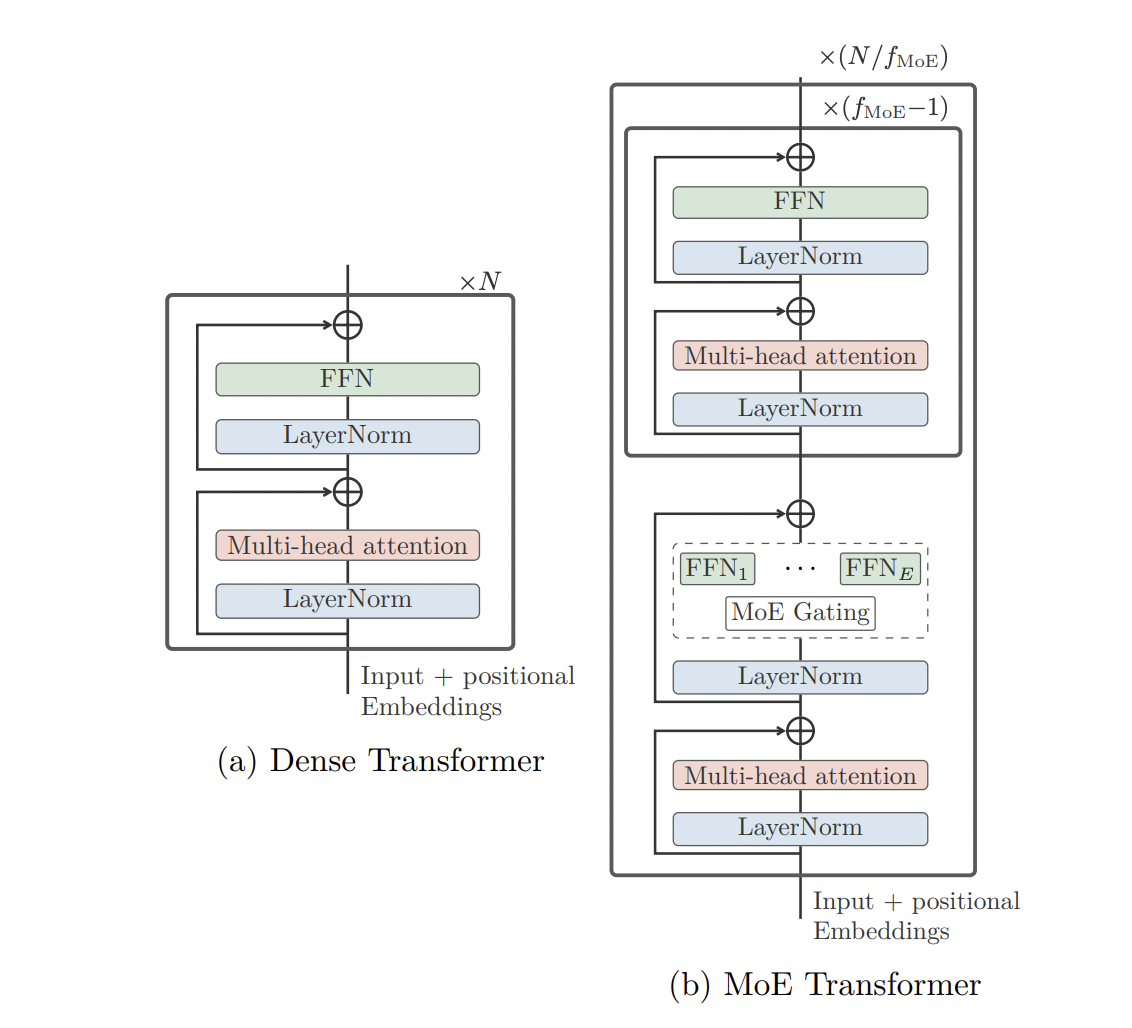
\includegraphics[width=0.7\linewidth]{images/nllb.png}
    \caption{NLLB pipeline \cite{nllb200-2020}}
    \label{fig:nllb}
\end{figure}

Figure \ref{fig:nllb} shows the Dense Transformer and MoE Transformer layers implemented within the model. MoE \cite{masoudnia-2012-moe} utilises a gating mechanism to route different inputs to different subsets of experts (sub-networks), allowing the model to handle various linguistic phenomena efficiently. Additionally, the model is then trained on a diverse set of languages, complemented with back-translation and data augmentation to generate additional data for low-resource languages \cite{nllb200-2020}.

% The original paper is 192 pages long and impossible to be dissected in just one section.


\subsection{Evaluation Metrics}

In this study, BLEU \cite{papieni-2002-bleu}, SacreBLEU \cite{post-2018-sacrebleu}, and METEOR \cite{lavie-2007-meteor} are applied as evaluation metrics due to their popularity, simplicity, and ease-of-use. While other metrics such as Crosslingual Optimized Metric for Evaluation of Translation (COMET) \cite{rei-2020-comet} and BERTSCore \cite{zhang-2020-bertscore} exist, they involve using a deep neural network or a transformer to evaluate, which naturally increase computational cost and slow down calculation greatly.

\subsubsection{BLEU}

Bilingual Evaluation Understudy (BLEU) \cite{papieni-2002-bleu} is the most commonly used metric for machine translation (MT). It assesses how well a candidate translation matches the reference translation using precision metrics for n-grams and incorporates a brevity penalty to prevent overly short translations from achieving high scores.

The BLEU score is calculated as:
\begin{equation}
    \text{BLEU} = BP \cdot \exp \left( \sum_{n=1}^{N} w_n \log p_n \right)
\end{equation}
where \( BP \) is the brevity penalty, \( p_n \) is the precision for n-grams, and \( w_n \) is the weight for each n-gram (often uniformly distributed, so \( w_n = \frac{1}{N} \)).

The brevity penalty (BP) is calculated as:
\begin{equation}
    BP = \begin{cases}
        1                     & \text{if } c > r    \\
        e^{(1 - \frac{r}{c})} & \text{if } c \leq r
    \end{cases}
\end{equation}
where \( c \) is the length of the candidate translation and \( r \) is the effective reference length.

The n-gram precision, as presented in the original BLEU paper \cite{papieni-2002-bleu}, is calculated as:
\begin{equation}
    p_n = \frac{\sum_{C \in \{Candidates\}} \sum_{\text{n-gram} \in C} \text{Count}_{\text{clip}}(\text{n-gram})}{\sum_{C \in \{Candidates\}} \sum_{\text{n-gram} \in C} \text{Count}(\text{n-gram})}
\end{equation}
where \( p_n \) is the precision for n-grams, \( \sum_{C \in \{Candidates\}} \) denotes the summation over all candidate translations, \( \sum_{\text{n-gram} \in C} \) denotes the summation over all n-grams in a candidate translation \( C \). \( \text{Count}_{\text{clip}}(\text{n-gram}) \) is the clipped count of the n-gram, which is the count of the n-gram in the candidate translation limited by the maximum count of that n-gram in any reference translation. \( \text{Count}(\text{n-gram}) \) is the count of the n-gram in the candidate translation.

The machine translation community relies heavily upon the BLEU score, despite its several drawbacks. The metric has been reported to not correlate strongly with human judgement, showing variations in translation that could mean that a higher BLEU score does not necessarily indicate a true enhancement in translation quality \cite{callison-burch-2006-reevaluating-bleu}. Furthermore, the metric is tokenisation-dependant, making it challenging to directly compare BLEU scores between paper \cite{post-2018-sacrebleu}. Thus, the author proposed a standardised variant called SacreBLEU \cite{post-2018-sacrebleu}, which is essentially a Python script that applies its own metric-internal preprocessing and produces the same values as WMT \cite{barrault-2020-wmt}, utilising the WMT (2008–2018) and IWSLT 2017 \cite{cettolo-etal-2017-iwslt} test sets.

\subsubsection{METEOR}

Metric for Evaluation of Translation with Explicit ORdering (METEOR) \cite{lavie-2007-meteor} assesses a translation by calculating a score that reflects explicit word-to-word matches between the reference and a candidate translation \cite{agarwal-2008-meteor-mbleu-mter}. It is designed to address some limitations of the BLEU score, allowing matches between simple morphological variants and synonyms. The formula is defined as:
\begin{equation}
    \text{METEOR} = (1 - \gamma \cdot \text{frag}) \cdot \frac{P \cdot R}{\alpha \cdot P + (1 - \alpha) \cdot R}
\end{equation}
where \(P\) is the precision, \(R\) is the recall, and \(\text{frag}\) is the fragmentation penalty. \(\gamma\) is a parameter that controls the weight of the fragmentation penalty, commonly set to 0.5, and \(\alpha\) is a parameter that controls the balance between precision and recall, commonly set to 0.9,

\subsection{Inference Details}

OPUS-MT models are taken from the Helsinki-NLP repository through the Hugging Face website \cite{huggingface,zhang-2023-fine-tuning} with the exception of Hebrew-to-English models taken directly from 'tiedeman/opus-mt-he-en'. The 'mbart-large-50-many-to-many-mmt', the 'm2m100\_418M', and the 'nllb-200-distilled-600M' model variants are used for mBART-50 \cite{liu-2020-mbart}, M2M-100 \cite{fan-2020-m2m100}, and NLLB-200 \cite{nllb200-2020}, respectively. Similarly, all multilingual models are downloaded using the transformers \cite{wolf-2020-transformers} library from Hugging Face \cite{huggingface}. A batch size of 4 is used in all models. Translations from each source language to english are first generated through inference and saved into CSV files, before calculating the metrics score.

For BLEU and METEOR, tokenisation and metrics calculation use the NLTK \cite{bird-2009-natural} package, specifically:
\begin{itemize}
    \item \texttt{nltk.word\_tokenize} \\
    \item \texttt{nltk.translate.meteor\_score} \\
    \item \texttt{nltk.translate.bleu\_score.corpus\_bleu}
\end{itemize}
Additionally, the smoothing method 7 is used for the BLEU calculation, which interpolates two other smoothing functions: smoothing method 4, which divides by \( \frac{1}{\ln(\text{len}(T))} \), where \( T \) is the length of the translation; and smoothing method 5, which averages the \( n-1 \), \( n \), and \( n+1 \) gram matched counts \cite{nltk-bleu-docs}. The \texttt{sacrebleu} \cite{post-2018-sacrebleu} package from pip is used to calculate SacreBLEU \cite{post-2018-sacrebleu}.

All codes are written in Python 3.12.2 and run locally on MacOS Sonoma 14.4.1 with an M2 chip and 16 GB memory. Datasets and scripts will be available on GitHub: \url{https://github.com/stefanliemawan/eval-machine-translation}

\section{Evaluation}

\begin{table}[htbp]
    \centering
    \begin{minipage}{0.49\linewidth}
        \footnotesize
        \begin{tabular}{lrrr}
            \hline
            \textbf{Language} & \textbf{BLEU}   & \textbf{SacreBLEU} & \textbf{METEOR} \\
            \hline
            Chinese           & 0.0971          & \textit{59.5098}   & 0.7953          \\
            Dutch             & 0.0974          & 69.8803            & 0.8471          \\
            Finnish           & 0.0965          & 66.6267            & 0.8296          \\
            French            & 0.0967          & 69.8185            & 0.8357          \\
            German            & 0.0969          & 69.7422            & 0.8419          \\
            Hebrew            & 0.0977          & 66.5149            & 0.8229          \\
            Italian           & 0.0979          & 74.1298            & 0.8584          \\
            Japanese          & 0.0960          & 63.1435            & \textit{0.7893} \\
            Polish            & \textit{0.0952} & 61.9026            & 0.8425          \\
            Russian           & 0.0974          & 66.7046            & 0.8179          \\
            Spanish           & 0.0979          & 71.4174            & 0.8463          \\
            Turkish           & \textbf{0.0980} & 72.6551            & 0.8460          \\
            Ukrainian         & 0.0978          & \textbf{75.4447}   & \textbf{0.8667} \\
            \hline
        \end{tabular}
        \caption{OPUS-MT result.}
        \label{table:opus_result}
    \end{minipage}
    \begin{minipage}{0.49\linewidth}
        \footnotesize
        \begin{tabular}{lrrr}
            \hline
            \textbf{Language} & \textbf{BLEU}   & \textbf{SacreBLEU} & \textbf{METEOR} \\
            \hline
            Chinese           & 0.0962          & 54.7322            & 0.7600          \\
            Dutch             & 0.0970          & 63.6482            & 0.8007          \\
            Finnish           & 0.0963          & 47.2194            & 0.7067          \\
            French            & 0.0968          & 57.2482            & 0.7598          \\
            German            & 0.0967          & 63.1666            & 0.8022          \\
            Hebrew            & 0.0972          & 58.0846            & 0.7590          \\
            Italian           & 0.0972          & \textbf{65.9415}   & \textbf{0.8068} \\
            Japanese          & 0.0943          & 43.9547            & 0.7151          \\
            Polish            & \textbf{0.0978} & 62.7550            & 0.7923          \\
            Russian           & 0.0974          & 58.8820            & 0.7686          \\
            Spanish           & \textit{0.0883} & \textit{35.1593}   & 0.7306          \\
            Turkish           & 0.0975          & 50.9377            & \textit{0.6982} \\
            Ukrainian         & 0.0964          & 55.8637            & 0.7496          \\
            \hline
        \end{tabular}
        \caption{mBART50 result.}
        \label{table:mbart_result}
    \end{minipage}
\end{table}

\begin{table}[htbp]
    \centering
    \begin{minipage}{0.49\linewidth}
        \footnotesize
        \begin{tabular}{lrrr}
            \hline
            \textbf{Language} & \textbf{BLEU}   & \textbf{SacreBLEU} & \textbf{METEOR} \\
            \hline
            Chinese           & 0.0975          & 43.3490            & 0.6848          \\
            Dutch             & 0.0976          & 52.6920            & \textbf{0.7448} \\
            Finnish           & 0.0975          & 49.9149            & 0.7145          \\
            French            & 0.0969          & 51.4090            & 0.7288          \\
            German            & 0.0969          & 52.7877            & 0.7423          \\
            Hebrew            & 0.0981          & 50.3287            & 0.7198          \\
            Italian           & 0.0975          & \textbf{53.1644}   & 0.7341          \\
            Japanese          & \textit{0.0959} & \textit{41.6610}   & \textit{0.6511} \\
            Polish            & \textbf{0.0984} & 52.5151            & 0.7301          \\
            Russian           & 0.0976          & 48.2725            & 0.7027          \\
            Spanish           & 0.0977          & 52.9323            & 0.7371          \\
            Turkish           & 0.0978          & 51.3009            & 0.7262          \\
            Ukrainian         & 0.0978          & 46.5555            & 0.6890          \\
            \hline
        \end{tabular}
        \caption{M2M-100 result.}
        \label{table:m2m_result}
    \end{minipage}
    \begin{minipage}{0.49\linewidth}
        \footnotesize
        \begin{tabular}{lrrr}
            \hline
            \textbf{Language} & \textbf{BLEU}   & \textbf{SacreBLEU} & \textbf{METEOR} \\
            \hline
            Chinese           & \textbf{0.0949} & \textbf{50.4454}   & \textbf{0.7180} \\
            Dutch             & 0.0915          & 20.8988            & 0.2899          \\
            Finnish           & 0.0921          & 32.3926            & 0.4006          \\
            French            & 0.0950          & 32.1389            & 0.4338          \\
            German            & 0.0903          & 7.1436             & 0.1528          \\
            Hebrew            & 0.0897          & 2.3455             & 0.1412          \\
            Italian           & 0.0926          & 24.2702            & 0.3059          \\
            Japanese          & \textit{0.0842} & \textit{1.9569}    & \textit{0.0919} \\
            Polish            & 0.0937          & 38.4395            & 0.4739          \\
            Russian           & 0.0918          & 20.6734            & 0.2977          \\
            Spanish           & 0.0929          & 26.3313            & 0.3578          \\
            Turkish           & 0.0945          & 45.2721            & 0.6187          \\
            Ukrainian         & 0.0914          & 9.0340             & 0.1613          \\
            \hline
        \end{tabular}
        \caption{NLLB-200 result.}
        \label{table:nllb_result}
    \end{minipage}
\end{table}

Table \ref{table:opus_result}, \ref{table:mbart_result}, \ref{table:m2m_result}, and \ref{table:nllb_result}, and  shows the result from all four PTMs. All models perform similarly low on BLEU score across all languages, with NLLB-200 reaching 0.01 below on Japanese translation. The BLEU scores are very low (below 10 BLEU) in all cases due to the sentences being short (find cite). This also highlights the superiority of SacreBLEU compared to the flawed, standard BLEU.

% BLEU is notoriously unreliable for very short texts. The score will be disproportionately influenced by small differences if there isn't much text to begin with because there is a Brevity Penalty set in place to discourage the model from outputting fewer words and getting a high score. 

OPUS-MT model shows the best performance in all languages, consistently reaching mostly above 60 SacreBLEU and 0.8 METEOR. The highest-rated languages are Ukrainian-to-English translation with 75.44 SacreBLEU and 0.86 METEOR, while the lowest scores are achieved on Chinese-to-English translation: 59.50 SacreBLEU and Japanese-to-English: 0.78 METEOR.

The mBART-50 model is the second-best-performing PTM and the best-performing multilingual model, achieving the best SacreBLEU and METEOR score in Italian-to-English translation while suffering the most in Spanish-to-English (SacreBLEU) and Turkish-to-English (METEOR) translation. Interestingly, Spanish receives the worst score in SacreBLEU while it performs decently in METEOR, and Turkish performs well in SacreBLEU score but has the worst in METEOR. Additionally, the model slightly outperforms OPUS-MT in Polish-to-English translation on SacreBLEU score (0.85 higher).

Similarly, SacreBLEU for Italian-to-English translation outperforms other languages with the M2M-100 model, although Dutch-to-English surpasses Italian-to-English by 0.01 in METEOR score. Japanese received the worst score in both SacreBLEU and METEOR for this model. M2M-100 performs worse in SacreBLEU compared to mBART-50, but comparably similar in METEOR scores.

NLLB-200 scores much lower compared to other models in both SacreBLEU and METEOR in almost all languages. It scores highest in Chinese-to-English translation in all metrics, while showing significant variability among other languages. However, Japanese-to-English translation suffers with extremely low scores of 1.95 SacreBLEU and 0.09 METEOR. Additionally, German, Hebrew, and Ukrainian also have low SacreBLEU and METEOR scores, among the other languages.

\begin{figure}[htbp]
    \centering
    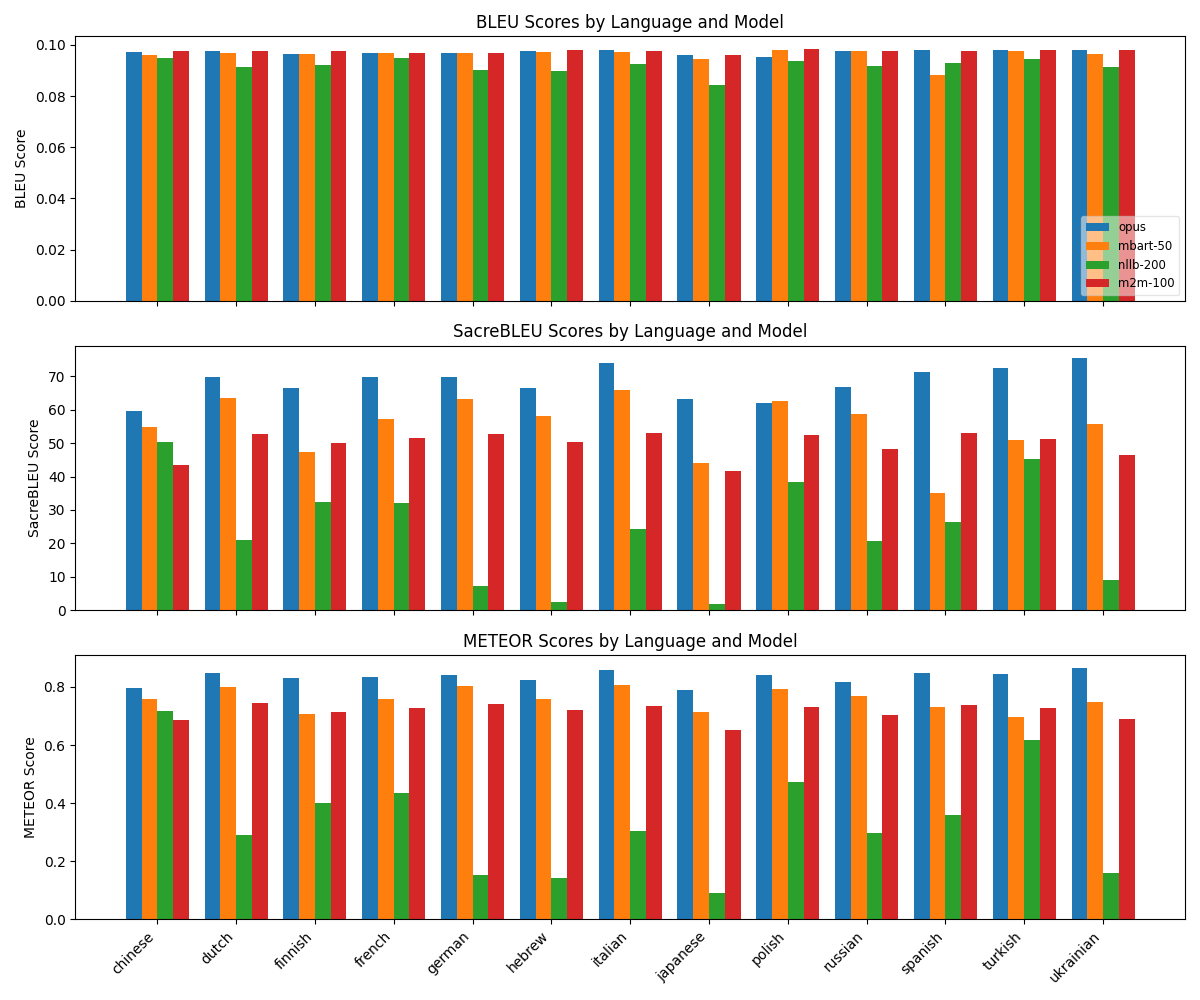
\includegraphics[width=1\linewidth]{figures/metrics_bar.png}
    \caption{BLEU, SacreBLEU, and METEOR scores of each model on each language pair.}
    \label{fig:result_visual}
\end{figure}

The BLEU, SacreBLEU, and METEOR scores gained by each model, categorised by every language pairs are illustrated in Figure \ref{fig:result_visual}. Dutch, Italian, and Ukrainian translations generally score higher across all metrics, suggesting that these languages are well-supported by the pre-trained models. Japanese translations, however, pose significant challenges for all models, as indicated by the consistently low scores across all metrics. Japanese-to-English translation seems to have the worst score on average across the four models, but particularly bad on multilingual models. In contrast, Dutch and German have consistently high results on all models except for NLLB-200, often reaching close to the highest language SacreBLEU and METEOR scores.

\begin{figure}[htbp]
    \centering
    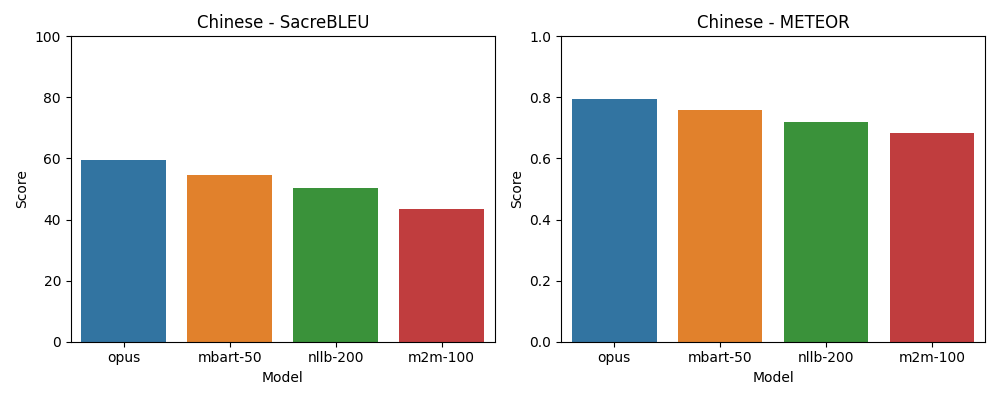
\includegraphics[width=0.49\linewidth]{figures/chinese_all_metrics.png}
    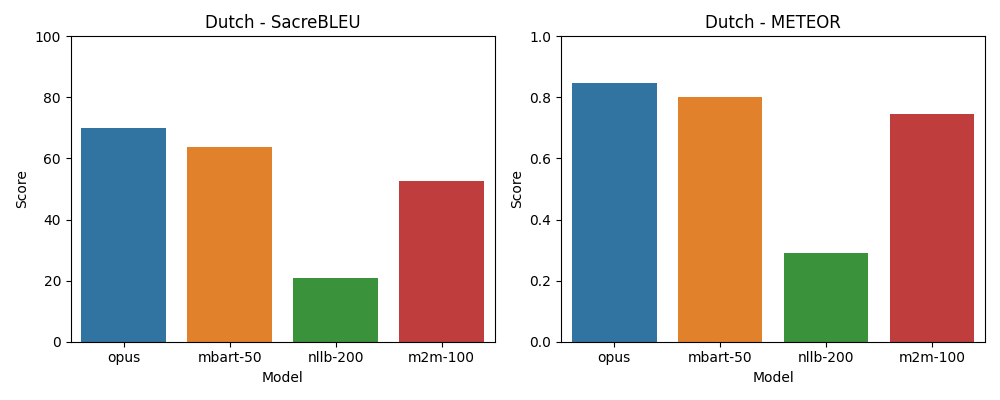
\includegraphics[width=0.49\linewidth]{figures/dutch_all_metrics.png}
    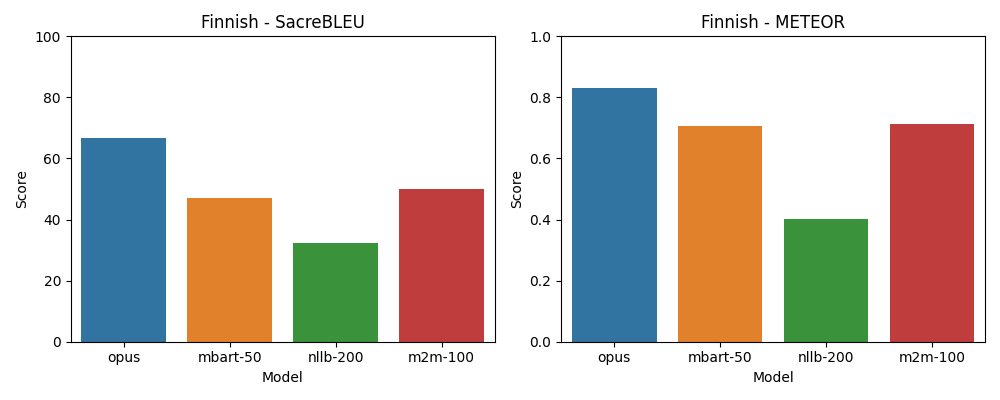
\includegraphics[width=0.49\linewidth]{figures/finnish_all_metrics.png}
    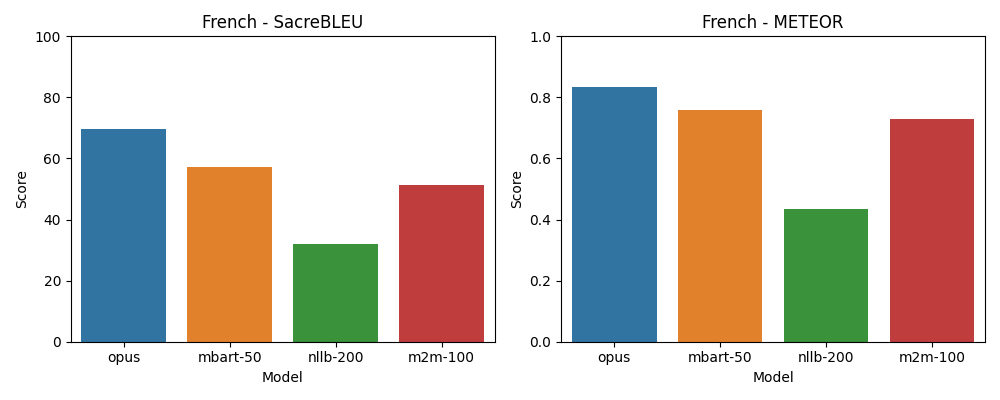
\includegraphics[width=0.49\linewidth]{figures/french_all_metrics.png}
    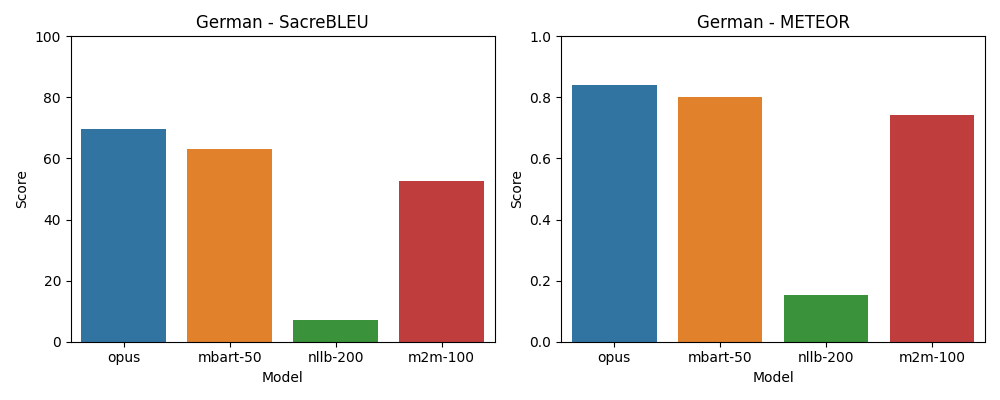
\includegraphics[width=0.49\linewidth]{figures/german_all_metrics.png}
    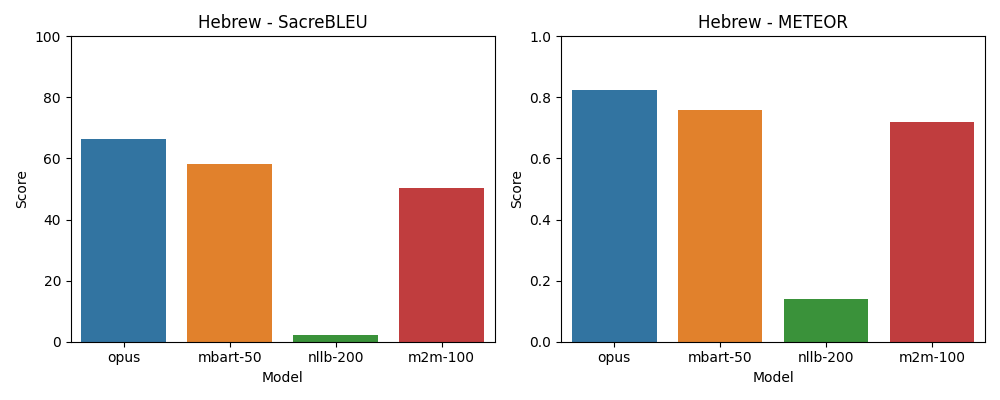
\includegraphics[width=0.49\linewidth]{figures/hebrew_all_metrics.png}
    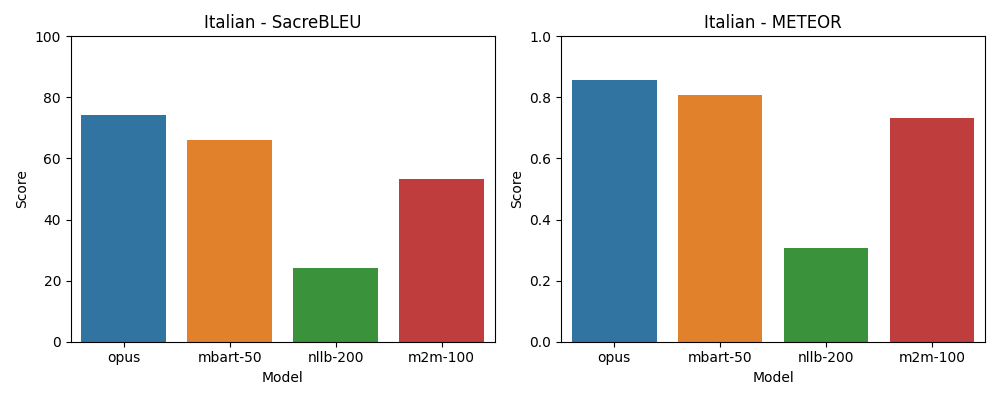
\includegraphics[width=0.49\linewidth]{figures/italian_all_metrics.png}
    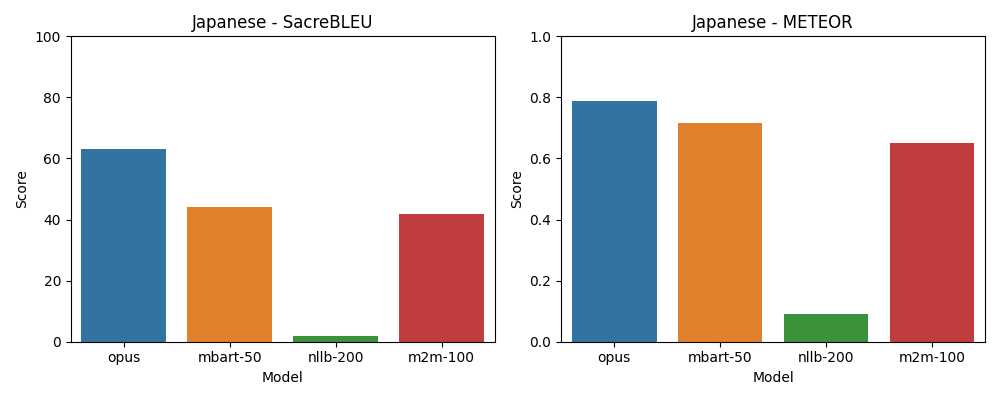
\includegraphics[width=0.49\linewidth]{figures/japanese_all_metrics.png}
    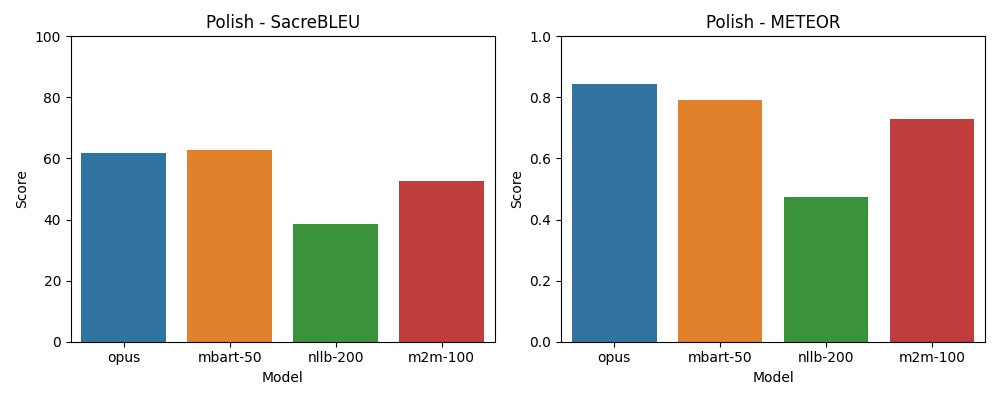
\includegraphics[width=0.49\linewidth]{figures/polish_all_metrics.png}
    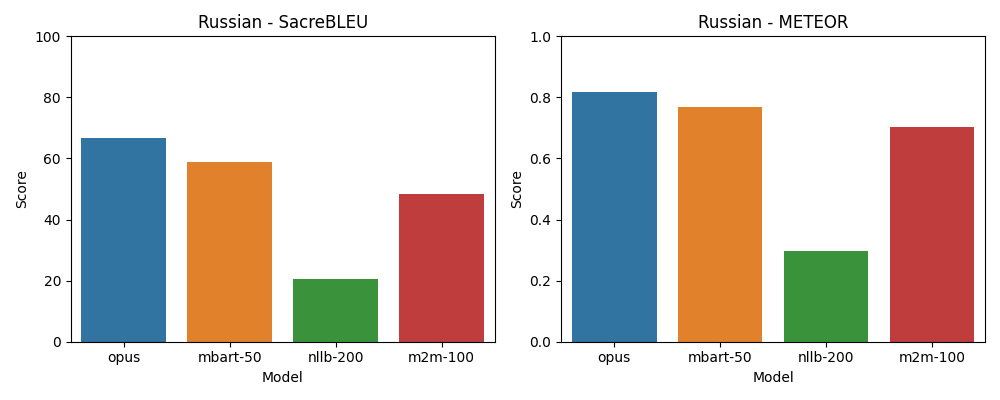
\includegraphics[width=0.49\linewidth]{figures/russian_all_metrics.png}
    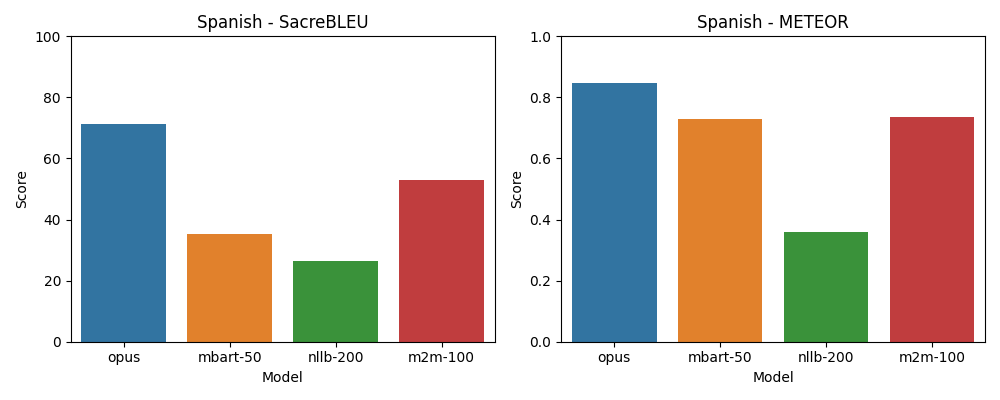
\includegraphics[width=0.49\linewidth]{figures/spanish_all_metrics.png}
    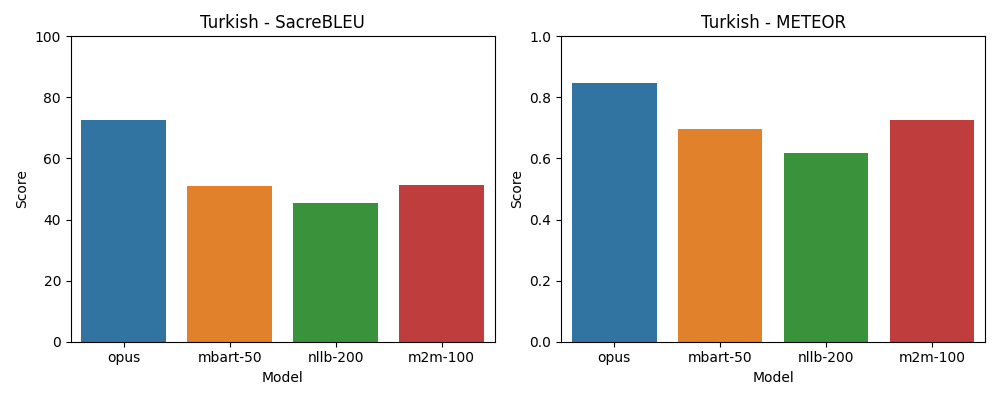
\includegraphics[width=0.49\linewidth]{figures/turkish_all_metrics.png}
    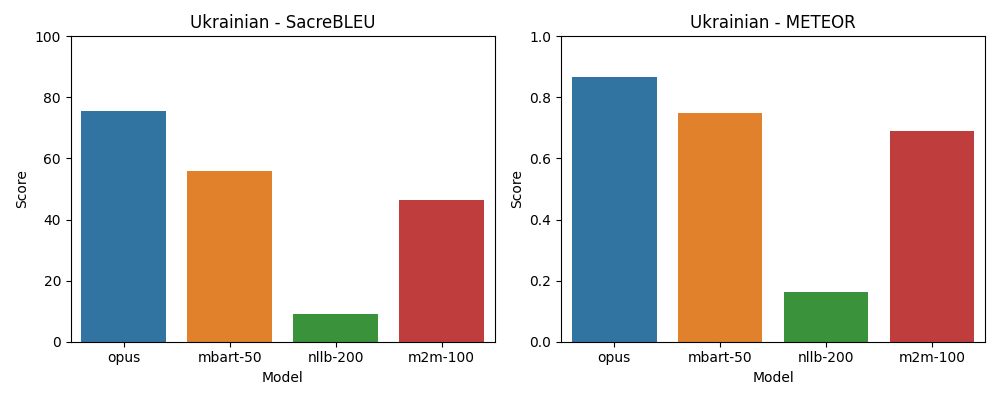
\includegraphics[width=0.49\linewidth]{figures/ukrainian_all_metrics.png}
    \caption{Performance of every language.}
    \label{fig:lang_metrics}
\end{figure}

Figure \ref{fig:lang_metrics} shows the SacreBLEU and METEOR scores for each language, categorised by model. The OPUS-MT and mBART-50 models are again shown as the clear winners in almost all languages. M2M-100 also performs competitively with mBART-50 in most languages, surpassing mBART-50 in Spanish-to-English translation. NLLB-200 is clearly shown to suffer greatly across all languages besides Chinese. All four models seem to perform consistently against each other in Chinese-to-English and Turkish-to-English translations.

\begin{figure}[htbp]
    \centering
    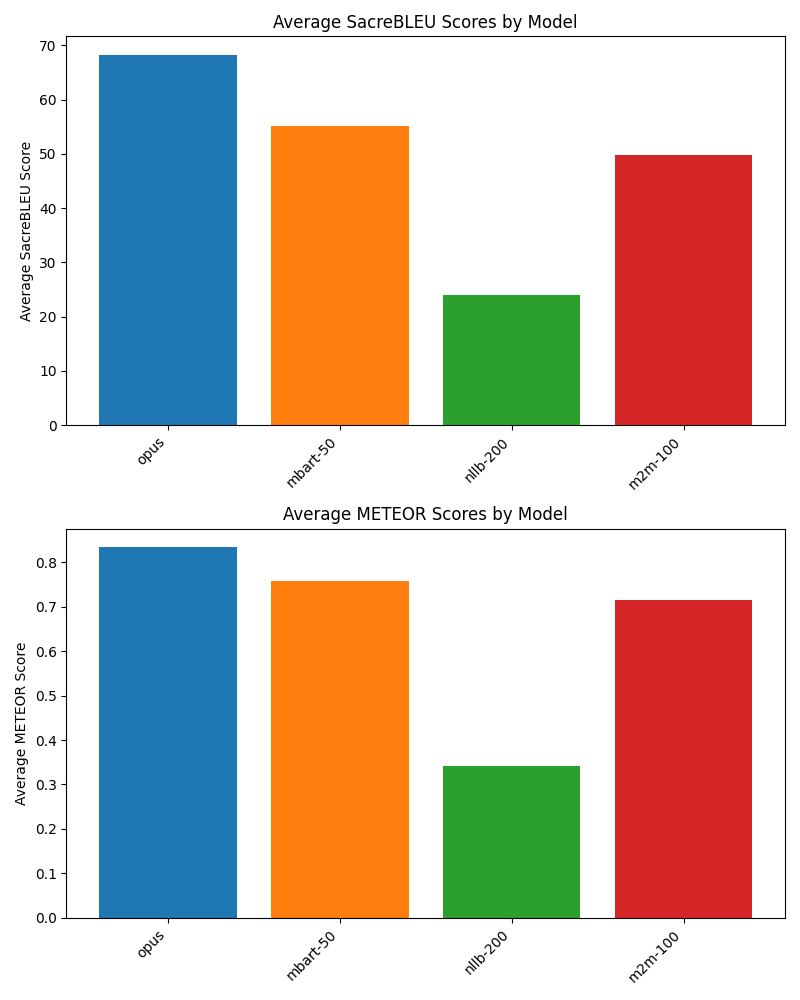
\includegraphics[width=0.49\linewidth]{figures/average_metrics_bar.png}
    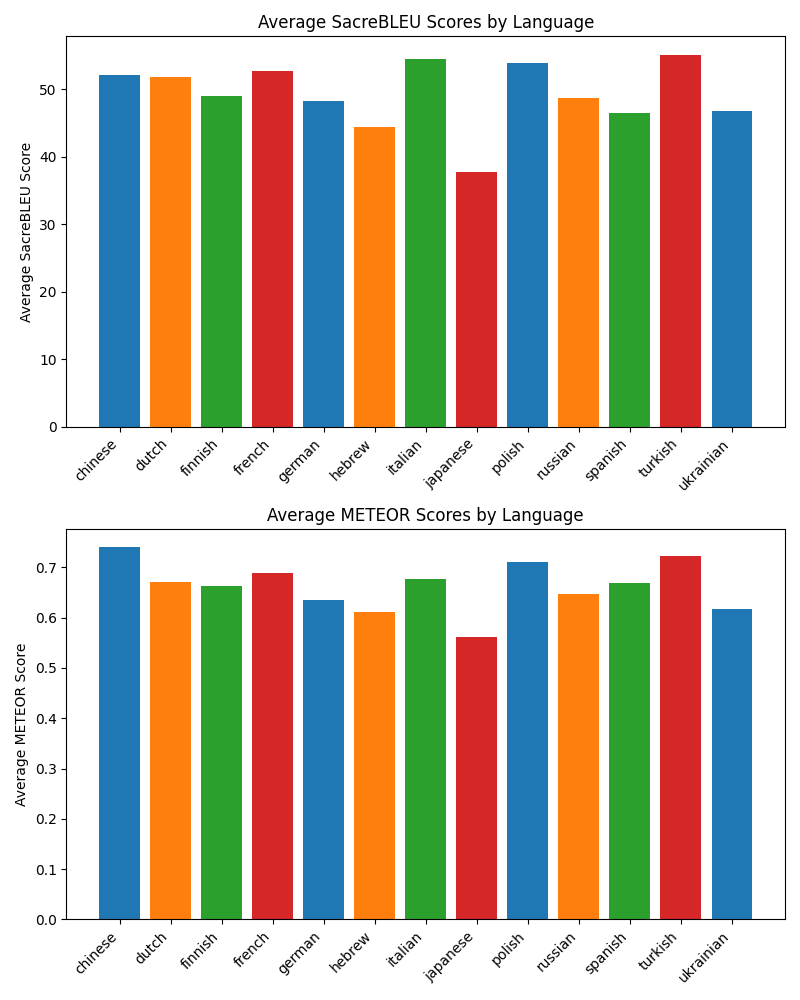
\includegraphics[width=0.49\linewidth]{figures/average_metrics_lang_bar.png}
    \caption{The average BLEU, SacreBLEU, and METEOR scores by model (left) and by language (right)}
    \label{fig:average_bars}
\end{figure}

Visualisations of the average SacreBLEU and METEOR, categorised by model (left figures) and language (right figures) is shown in Figure \ref{fig:average_bars}, providing a closer insight on how each model and language perform independently. It can be seen that when averaged across all languages, mBART-50 performs more closely to OPUS-MT on the METEOR score than the SacreBLEU score. Language-wise, Italian, Polish, and Turkish achieve the best average SacreBLEU scores while Chinese, Polish, and Turkish are the top three languages with the highest average METEOR scores.

\begin{figure}[htbp]
    \centering
    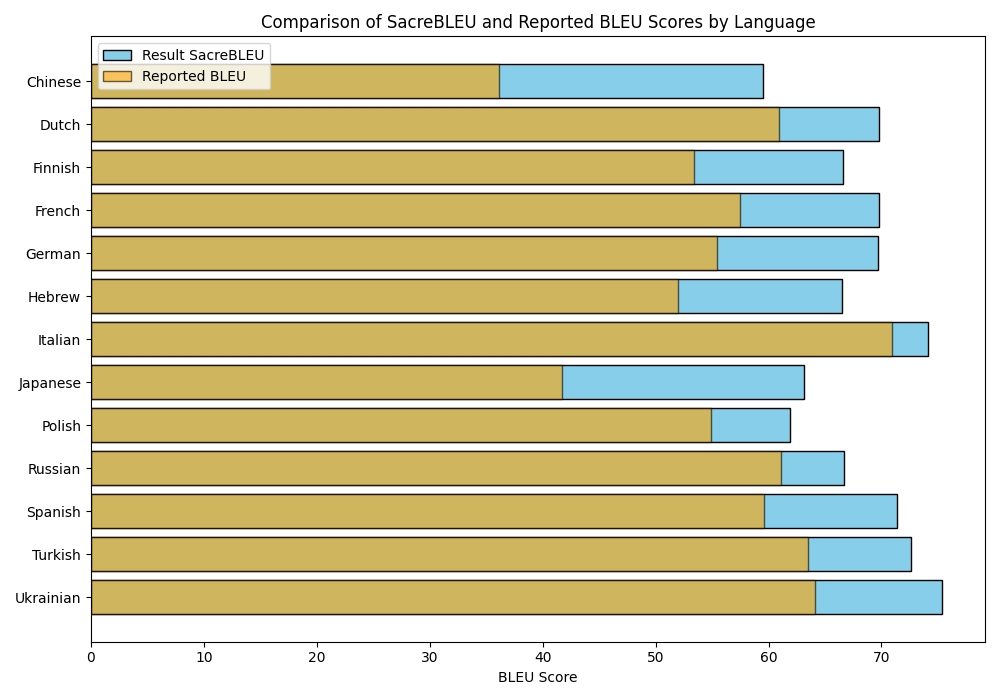
\includegraphics[width=0.8\linewidth]{figures/opus_bleu_comparison.png}
    \caption{Comparison between reported OPUS-MT models performance and performance in this experiment.}
    \label{fig:opus_comparison}
\end{figure}

Figure \ref{fig:opus_comparison} highlights the difference between each OPUS-MT model's reported BLEU scores compared to the SacreBLEU result of this study. The reported BLEU is evaluated on the Tatoeba dataset \cite{tiedemann-2020-opus-mt}. It can be seen that the scores are quite aligned, with Ukrainian and Italian reaching the two highest scores while Chinese, Polish, and Japanese suffer.

While this study's experiments resulted in a moderately higher overall SacreBLEU, the dataset used here is also significantly smaller than the full Tatoeba challenge dataset \cite{tiedemann-2020-tatoeba-challenge} that are used in the OPUS-MT reported BLEU. In contrast, this study employs the same set of parallel sentences for all languages, which should lead to more consistent results. Nevertheless, a direct comparison between these results is not fully pertinent.


\begin{table}[htbp]
    \centering
    \begin{tabular}{l r r}
        \hline
        \textbf{Language} & \textbf{SacreBLEU} & \textbf{Reported BLEU} \\
        \hline
        Chinese           & \textit{59.5}      & \textit{36.1}          \\
        Dutch             & 69.8               & 60.9                   \\
        Finnish           & 66.6               & 53.4                   \\
        French            & 69.8               & 57.5                   \\
        German            & 69.7               & 55.4                   \\
        Hebrew            & 66.5               & 52.0                   \\
        Italian           & 74.1               & 70.9                   \\
        Japanese          & 63.1               & 41.7                   \\
        Polish            & 61.9               & 54.9                   \\
        Russian           & 66.7               & 61.1                   \\
        Spanish           & 71.4               & 59.6                   \\
        Turkish           & 72.6               & 63.5                   \\
        Ukrainian         & \textbf{75.4}      & \textbf{64.1}          \\
        \hline
    \end{tabular}
    \caption{OPUS-MT result compared with reported BLEU result}
    \label{table:opus_comparison}
\end{table}

Additionally, Table \ref{table:opus_comparison} shows the full scores of both results SacreBLEU and reported BLEU from each OPUS-MT model \cite{tiedemann-2020-opus-mt}. The reported BLEU scores are taken from each model card in the HuggingFace repository \cite{huggingface}. Unfortunately, other models are not benchmarked on the Tatoeba dataset, not evaluated on the source languages used in this study, and use different metrics \cite{liu-2020-mbart,fan-2020-m2m100,nllb200-2020}, and therefore cannot be directly compared to the results of this study.

\begin{figure}[htbp]
    \centering
    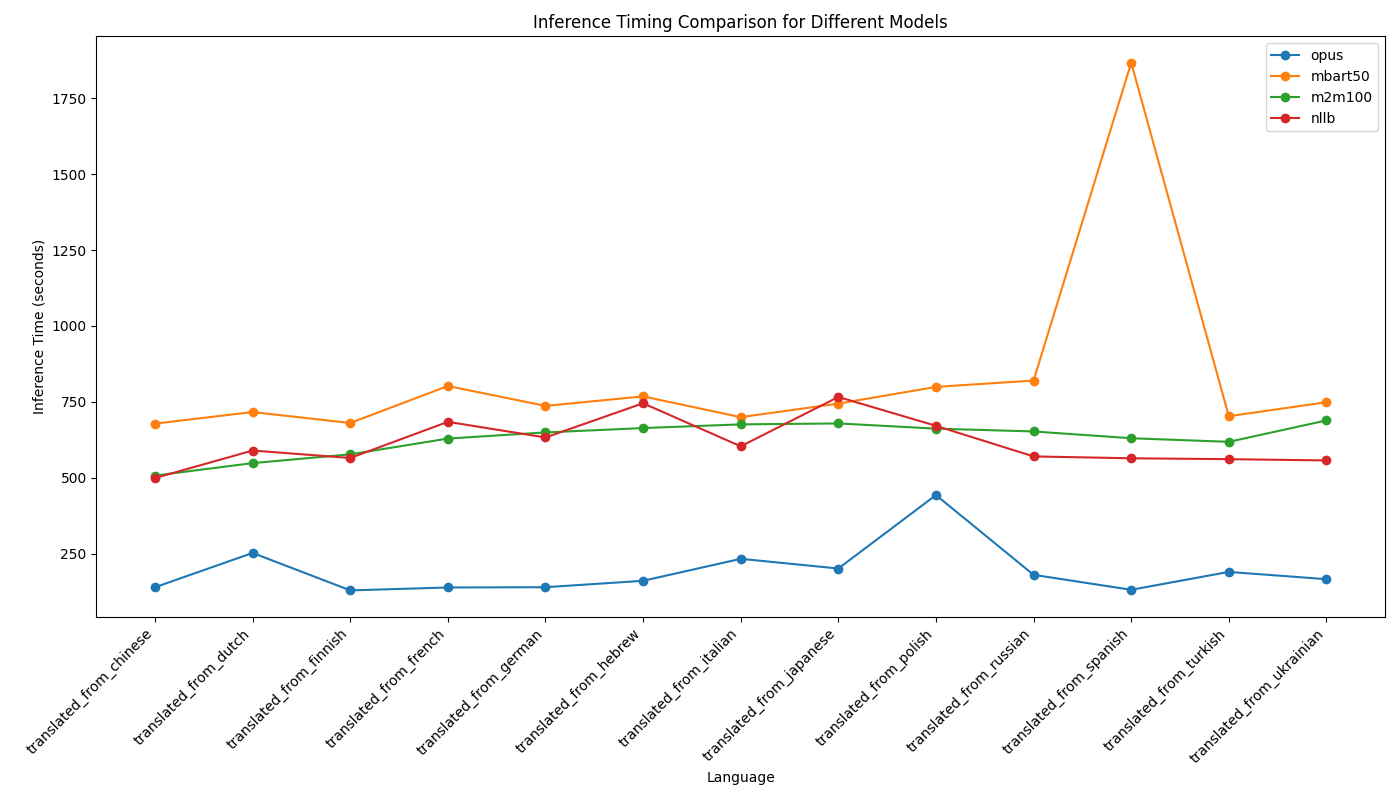
\includegraphics[width=0.9\linewidth]{figures/inference_timings.png}
    \caption{Inference timings for every model.}
    \label{fig:inference_timings}
\end{figure}

Lastly, Figure \ref{fig:inference_timings} shows the time taken to translate all 1,323 sentences for each language across experimented models. The OPUS-MT model is the fastest among the other three multilingual models. M2M-100 and NLLB-200 achieve similar timings, while mBART-50 has slightly longer timings on average. It is unknown why mBART50 suffers from a significantly higher timing on the Spanish-to-English translation. Re-running the experiment shows that this timing is consistent and not an anomaly.


\section{Conclusion}

This study's findings show that while multilingual models have been shown to achieve higher performance compared to one-to-one translation models \cite{liu-2020-mbart}, this does not hold on short sentences, many-to-English translations across the 14 source languages, with regard to unfine-tuned multilingual models in this study.

OPUS-MT achieves the best performance across all 14 languages. mBART-50 is the second-best-performing model, beating OPUS-MT only in Polish SacreBLEU. Nevertheless, both the mBART-50 and the M2M-100 models perform generally well in all languages. NLLB-200, however, achieves much lower scores in both SacreBLEU and METEOR for all languages except for Chinese, slightly outperforming M2M-100 but still slightly below mBART-50. NLLB-200 should then be avoided for use without any further fine-tuning on these languages. Note that that the distilled version is used in this study for NLLB-200 instead of the larger 3.3 billion parameters model variant.

Chinese, Italian, Polish, and Turkish have the best average scores over all four models. Ukrainian by OPUS-MT has the highest SacreBLEU and METEOR scores across all the other models and languages. These results show that these languages are well-supported within the four (MT-PTMs) evaluated in this study, achieving decent results without any fine-tuning.

\section{Discussion}

When the dataset is curated, only the first translation of the same English phrases is taken, the others are discarded. This ignores several possible translation references which may include synonyms or different phrasings, thus affecting the evaluation score, especially for BLEU and SacreBLEU metrics.

The dataset consists of mostly short sentences, with little or none linguistic depth. Whether the result of this study stays consistent for longer sentences or documents is not known and should be further looked into. The Tatoeba dataset \cite{tiedemann-2020-tatoeba-challenge} consisting of short sentences has been reported to be too optimistic when evaluated with other datasets that are more realistic \cite{tiedemann-2020-opus-mt}.

As Tatoeba \cite{tatoeba} is run mostly by volunteers, there are also several limitations with its corpus. The quality of sentences can vary significantly depending on the contributors' language proficiency and the level of community engagement for specific languages. Moreover, not all sentences are reviewed or verified by native speakers or trusted users.

The languages chosen are mostly high-resource languages, while models such as NLLB-200 \cite{nllb200-2020} are specifically designed to address the problem with low-resource languages. Data leakage is also a possibility, as sentences included in this dataset are fairly common phrases, it is highly likely that the model has seen these during training.

Future works should incorporate more Pre-Trained Models (PTMs) and implement fine-tuning multilingual models for specific languages on languages-to-English translation as it can significantly improve performance \cite{zhang-2023-fine-tuning}. Furthermore, it may be beneficial to consider more general multilingual PTMs such as mBERT \cite{wu-2020-mbert-are-all} and PolyLM \cite{wei-2023-polylm}, which are trained for a wide range of NLP tasks instead of just machine translation.

\printbibliography
\end{document}
